% ACNS-ISC 2026 Submission — Springer LNCS Format
% Double-blind: no author information
\documentclass[runningheads]{llncs}

\usepackage[T1]{fontenc}
\usepackage{graphicx}
\usepackage{amsmath,amssymb}
\usepackage{hyperref}
\usepackage{color}
\renewcommand\UrlFont{\color{blue}\rmfamily}
\urlstyle{rm}

\begin{document}

\title{Bridging the Gap Between Theory and Practice in Adversarial Machine Learning: A Systematic Analysis of 454 Papers (2022--2025)}
\titlerunning{Theory-Practice Gap in Adversarial ML}

% Double-blind: authors anonymized
\author{Anonymous Author(s)}
\authorrunning{Anonymous}
\institute{Anonymous Institution}

\maketitle

%==============================================================================
\begin{abstract}
Machine learning systems are increasingly deployed in security-critical contexts, yet a persistent gap separates academic adversarial machine learning (AML) research from real-world deployment needs. We systematically analyze 454 papers published from 2022 to 2025 across four leading security conferences (ACM CCS, IEEE S\&P, NDSS, and USENIX Security), applying and extending the framework introduced by Apruzzese et al.\ in ``Real Attackers Don't Compute Gradients.'' We introduce a quantitative Gap Score capturing six dimensions of impractical assumptions. Our findings reveal that 94.7\% [95\% CI: 92.3\%, 96.4\%] of papers do not evaluate on deployed systems, 67.8\% [63.4\%, 72.0\%] require gradient access, 63.2\% [58.7\%, 67.5\%] assume white-box threat models, and 80.4\% [76.5\%, 83.8\%] assume high query budgets, with no statistically significant improvement from 2022 to 2025 (all p $>$ 0.28). Cross-venue analysis shows all four conferences exhibit similar gap patterns (mean Gap Score 3.04 to 3.25 out of 6, p $>$ 0.20). We offer recommendations for researchers, conference organizers, practitioners, and funders. The complete coded dataset of all 454 papers is provided as supplementary material to enable replication and extension.

\keywords{Adversarial Machine Learning \and Theory-Practice Gap \and Systematic Review \and Threat Modeling \and Security Metrics.}
\end{abstract}

%==============================================================================
\section{Introduction}
\label{sec:intro}

In 2023, Apruzzese et al.~\cite{apruzzese2022real} documented a significant gap between academic adversarial machine learning (AML) research and practical security needs. Their central observation: academic attacks frequently assume adversaries can compute gradients through target models, while real-world attackers rarely have such access.

This paper asks: \emph{four years later, has the research community addressed these concerns?}

We systematically analyzed 454 adversarial ML papers published from 2022 through 2025 at ACM CCS (118 papers), IEEE S\&P (79), NDSS (49), and USENIX Security (208). Each paper was evaluated across dimensions capturing practical relevance: threat model realism, gradient and query requirements, real-system validation, and consideration of economic factors. We introduce a quantitative \emph{Gap Score} framework that reduces these dimensions to a tractable 0 to 6 scale for comparative analysis.

Our contributions are:
\begin{enumerate}
    \item A large-scale systematic analysis of 454 papers across four security venues, quantifying the theory-practice gap along six dimensions.
    \item A novel Gap Score framework for measuring divergence from practical deployment conditions.
    \item Temporal trend analysis showing the gap has not meaningfully narrowed from 2022 to 2025.
    \item Cross-venue comparison revealing that all four conferences exhibit similar gap patterns.
    \item Actionable recommendations for researchers, venues, practitioners, and funders.
\end{enumerate}

%==============================================================================
\section{Background and Motivation}
\label{sec:background}

AML research has established an arms race between increasingly sophisticated attacks and defenses~\cite{carlini2019evaluating,tramer2020adaptive}. Threat models range from white-box (full model access enabling gradient computation) to black-box (query-only access) to gray-box (partial knowledge). However, concerns about practical relevance have intensified. Grosse et al.~\cite{grosse2024practical} surveyed 271 industry practitioners finding that researchers frequently overestimate realistic attacker capabilities. Apruzzese et al.~\cite{apruzzese2022real} observed that academic attacks frequently assume gradient access, while real-world attackers almost never have white-box access. These studies motivate our large-scale quantitative measurement of whether the gap has narrowed.

%==============================================================================
\section{Methodology}
\label{sec:methodology}

We systematically reviewed all adversarial ML papers published from 2022 through 2025 at four premier security venues. Papers were identified through keyword searches (including ``adversarial,'' ``backdoor,'' ``poisoning,'' ``robustness'') across proceedings and digital libraries, supplemented by cross-referencing papers cited in Apruzzese et al.~\cite{apruzzese2022real}. Our dataset comprises 454 papers: ACM CCS contributed 118 (26.0\%), IEEE S\&P 79 (17.4\%), NDSS 49 (10.8\%), and USENIX Security 208 (45.8\%), spanning 89 papers from 2022, 136 from 2023, 198 from 2024, and 31 from 2025 (Fig.~\ref{fig:dataset}). Each paper was coded on dimensions adapted from Apruzzese et al.: research focus (G1: attack, defense, or both), attack type (G2: evasion, poisoning, privacy, or multiple), data domain (G4: images, text, audio, malware, or other), threat model (T1: white-box, black-box, or gray-box), gradient access (Q1), query budget (Q2: high $>$1000 or low), real-system testing (G7), code release (G6), and economic consideration (G5). The coding was performed using OpenAI's GPT-4o model (temperature=0) with structured prompts explicitly defining each dimension. For each paper, we extracted the full text using PyPDF2 and provided it to the model along with a fixed-format prompt requiring responses for all 12 dimensions. This AI-assisted approach enabled systematic analysis at scale, though it introduces potential classification errors discussed in our limitations.

\begin{figure}[htbp]
    \centering
    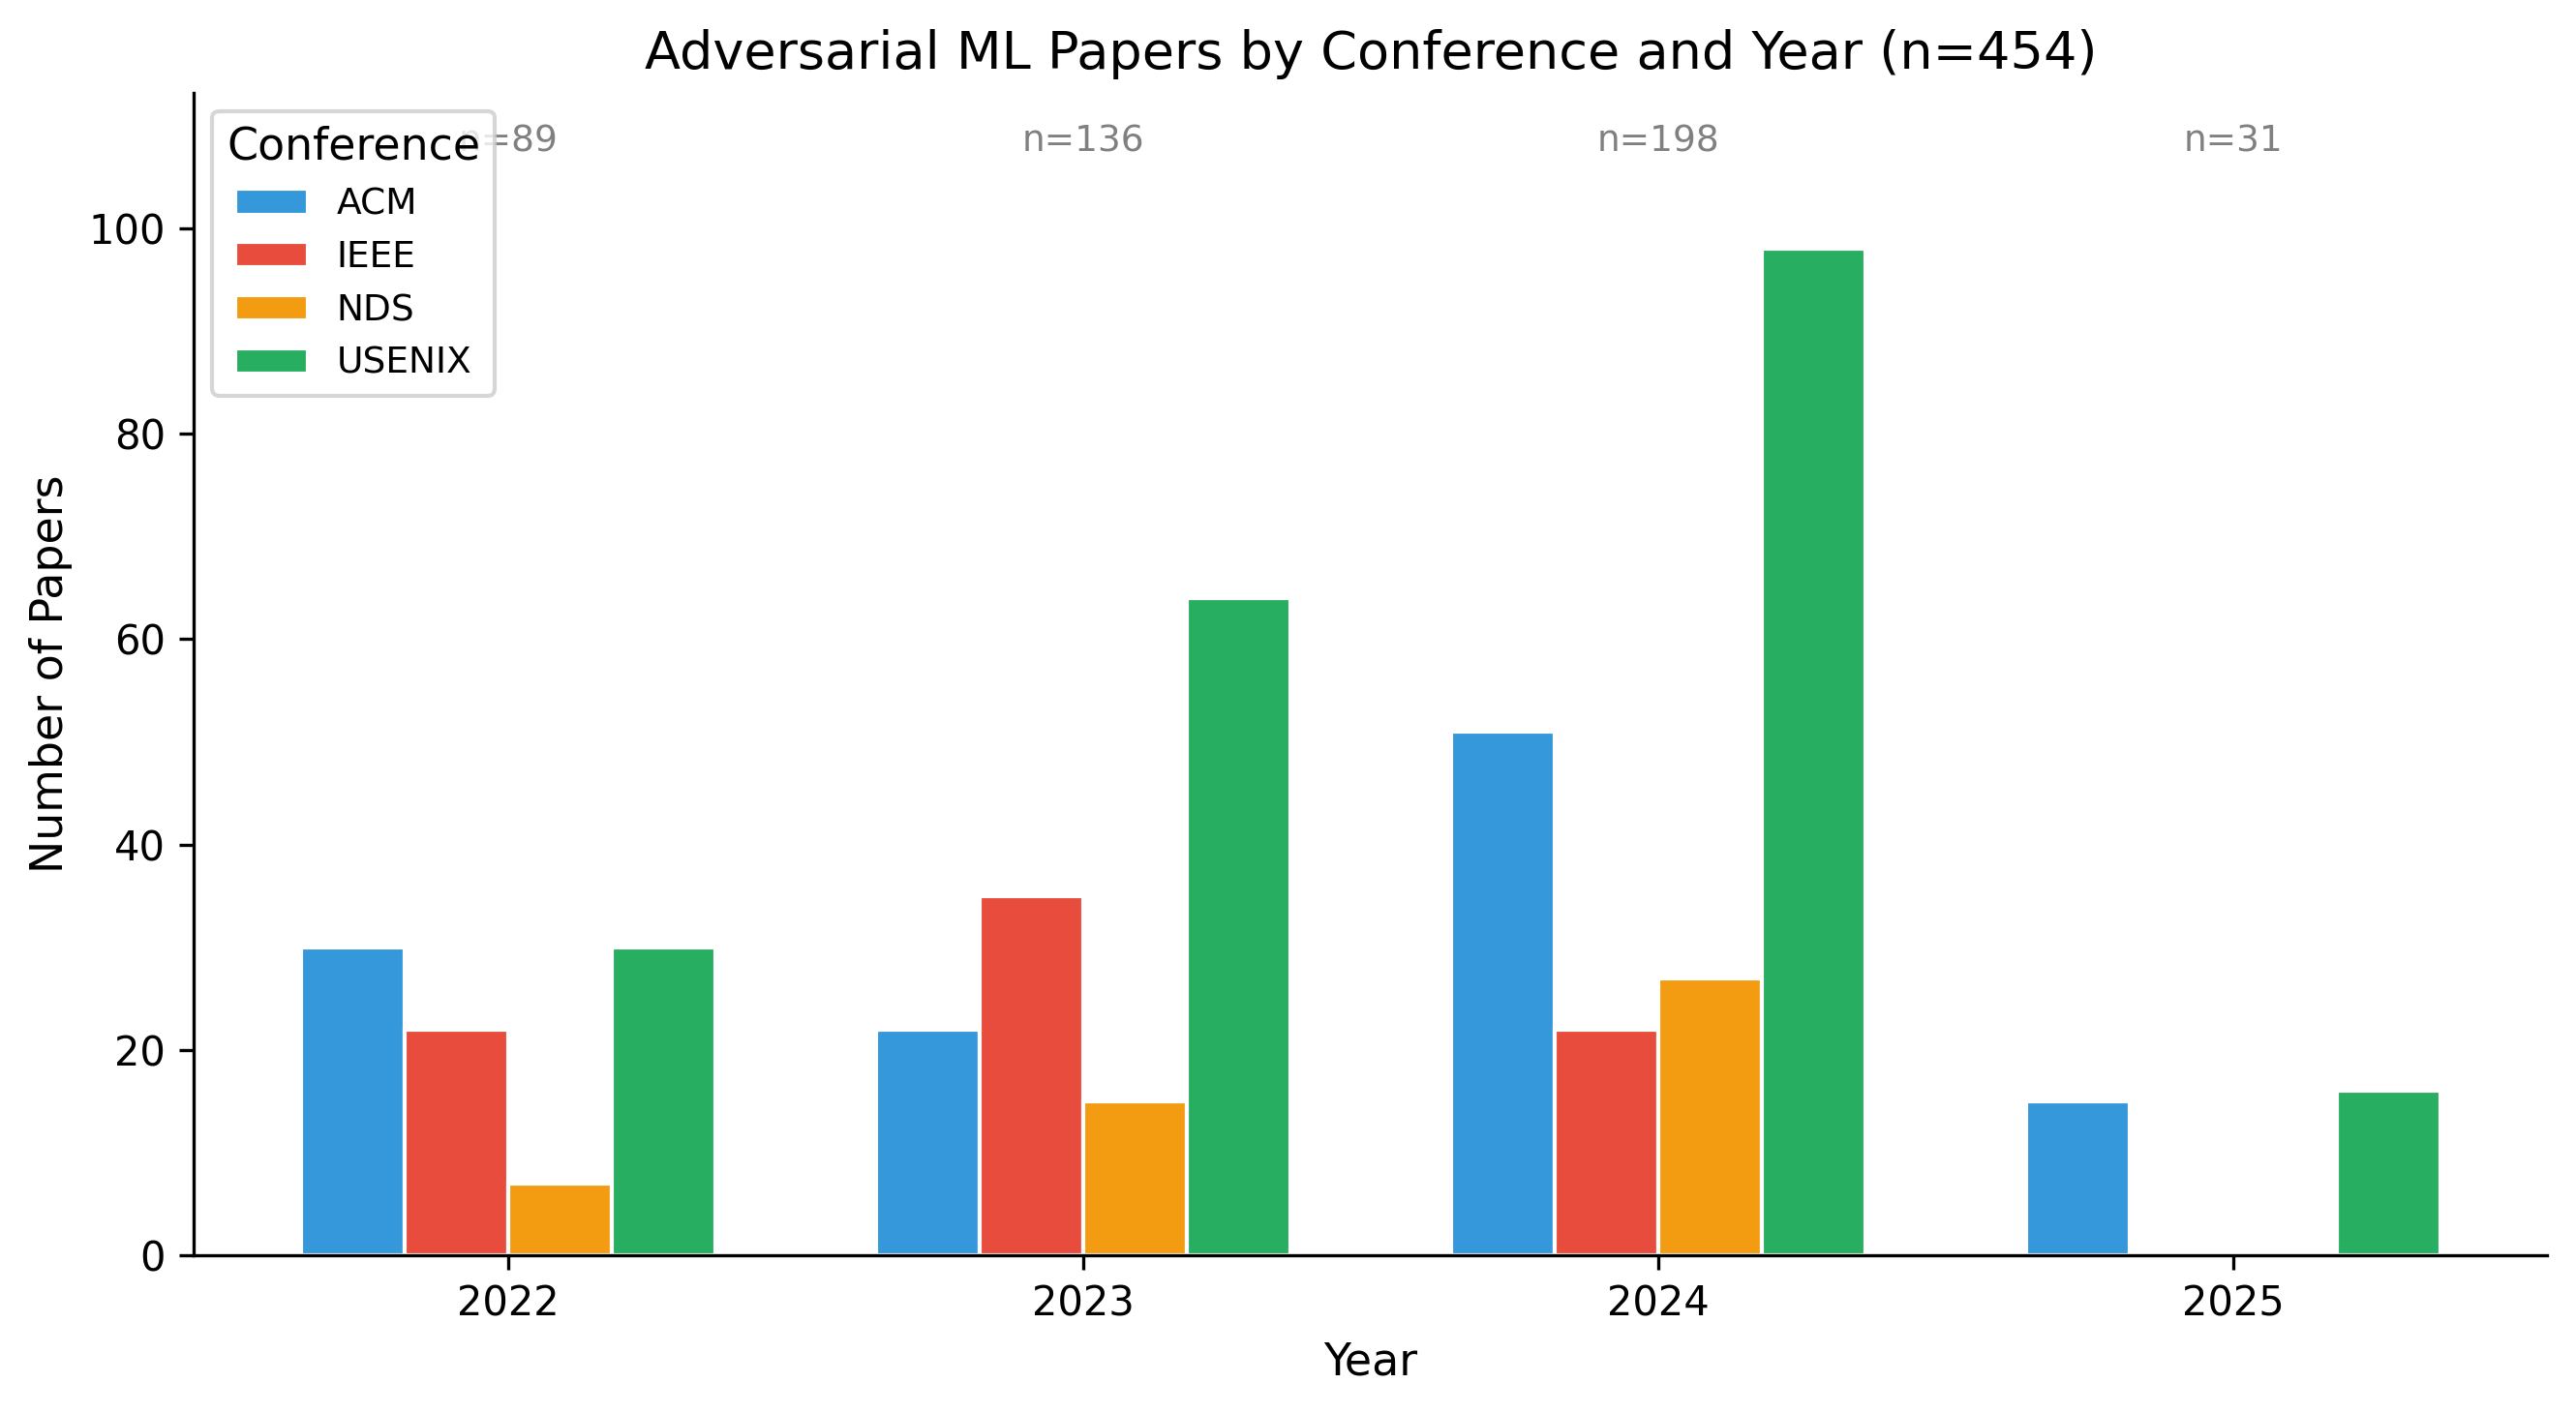
\includegraphics[width=\textwidth]{fig01_dataset_overview.png}
    \caption{Distribution of the 454 adversarial ML papers across four security conferences from 2022 through 2025}
    \label{fig:dataset}
\end{figure}

We computed a \emph{Gap Score} (0 to 6) summing six binary indicators: (1) white-box access, (2) gradient computation, (3) high query budget ($>$1000), (4) substantial computational resources ($>$100 GPU-hours), (5) no real-system testing, and (6) no economic consideration. Real-system testing requires production deployments with real users (laboratory testbeds do not qualify). White-box assumptions can be appropriate for open-source models, insider threats, or training-time attacks; our Gap Score flags potential misalignment with typical deployment constraints, not universal inappropriateness.

%==============================================================================
\section{Quantitative Findings}
\label{sec:findings}

Our analysis reveals several dimensions where research practices diverge from deployment realities. Figure~\ref{fig:gap_overview} summarizes the key gap indicators across all 454 papers. We report standalone results for five dimensions (real-world testing, gradient dependency, threat models, query budgets, and domain distribution); the computational resources dimension contributes to the Gap Score but is not reported separately as it correlates strongly with gradient access and is difficult to assess consistently across heterogeneous attack types and domains.

\begin{figure}[htbp]
    \centering
    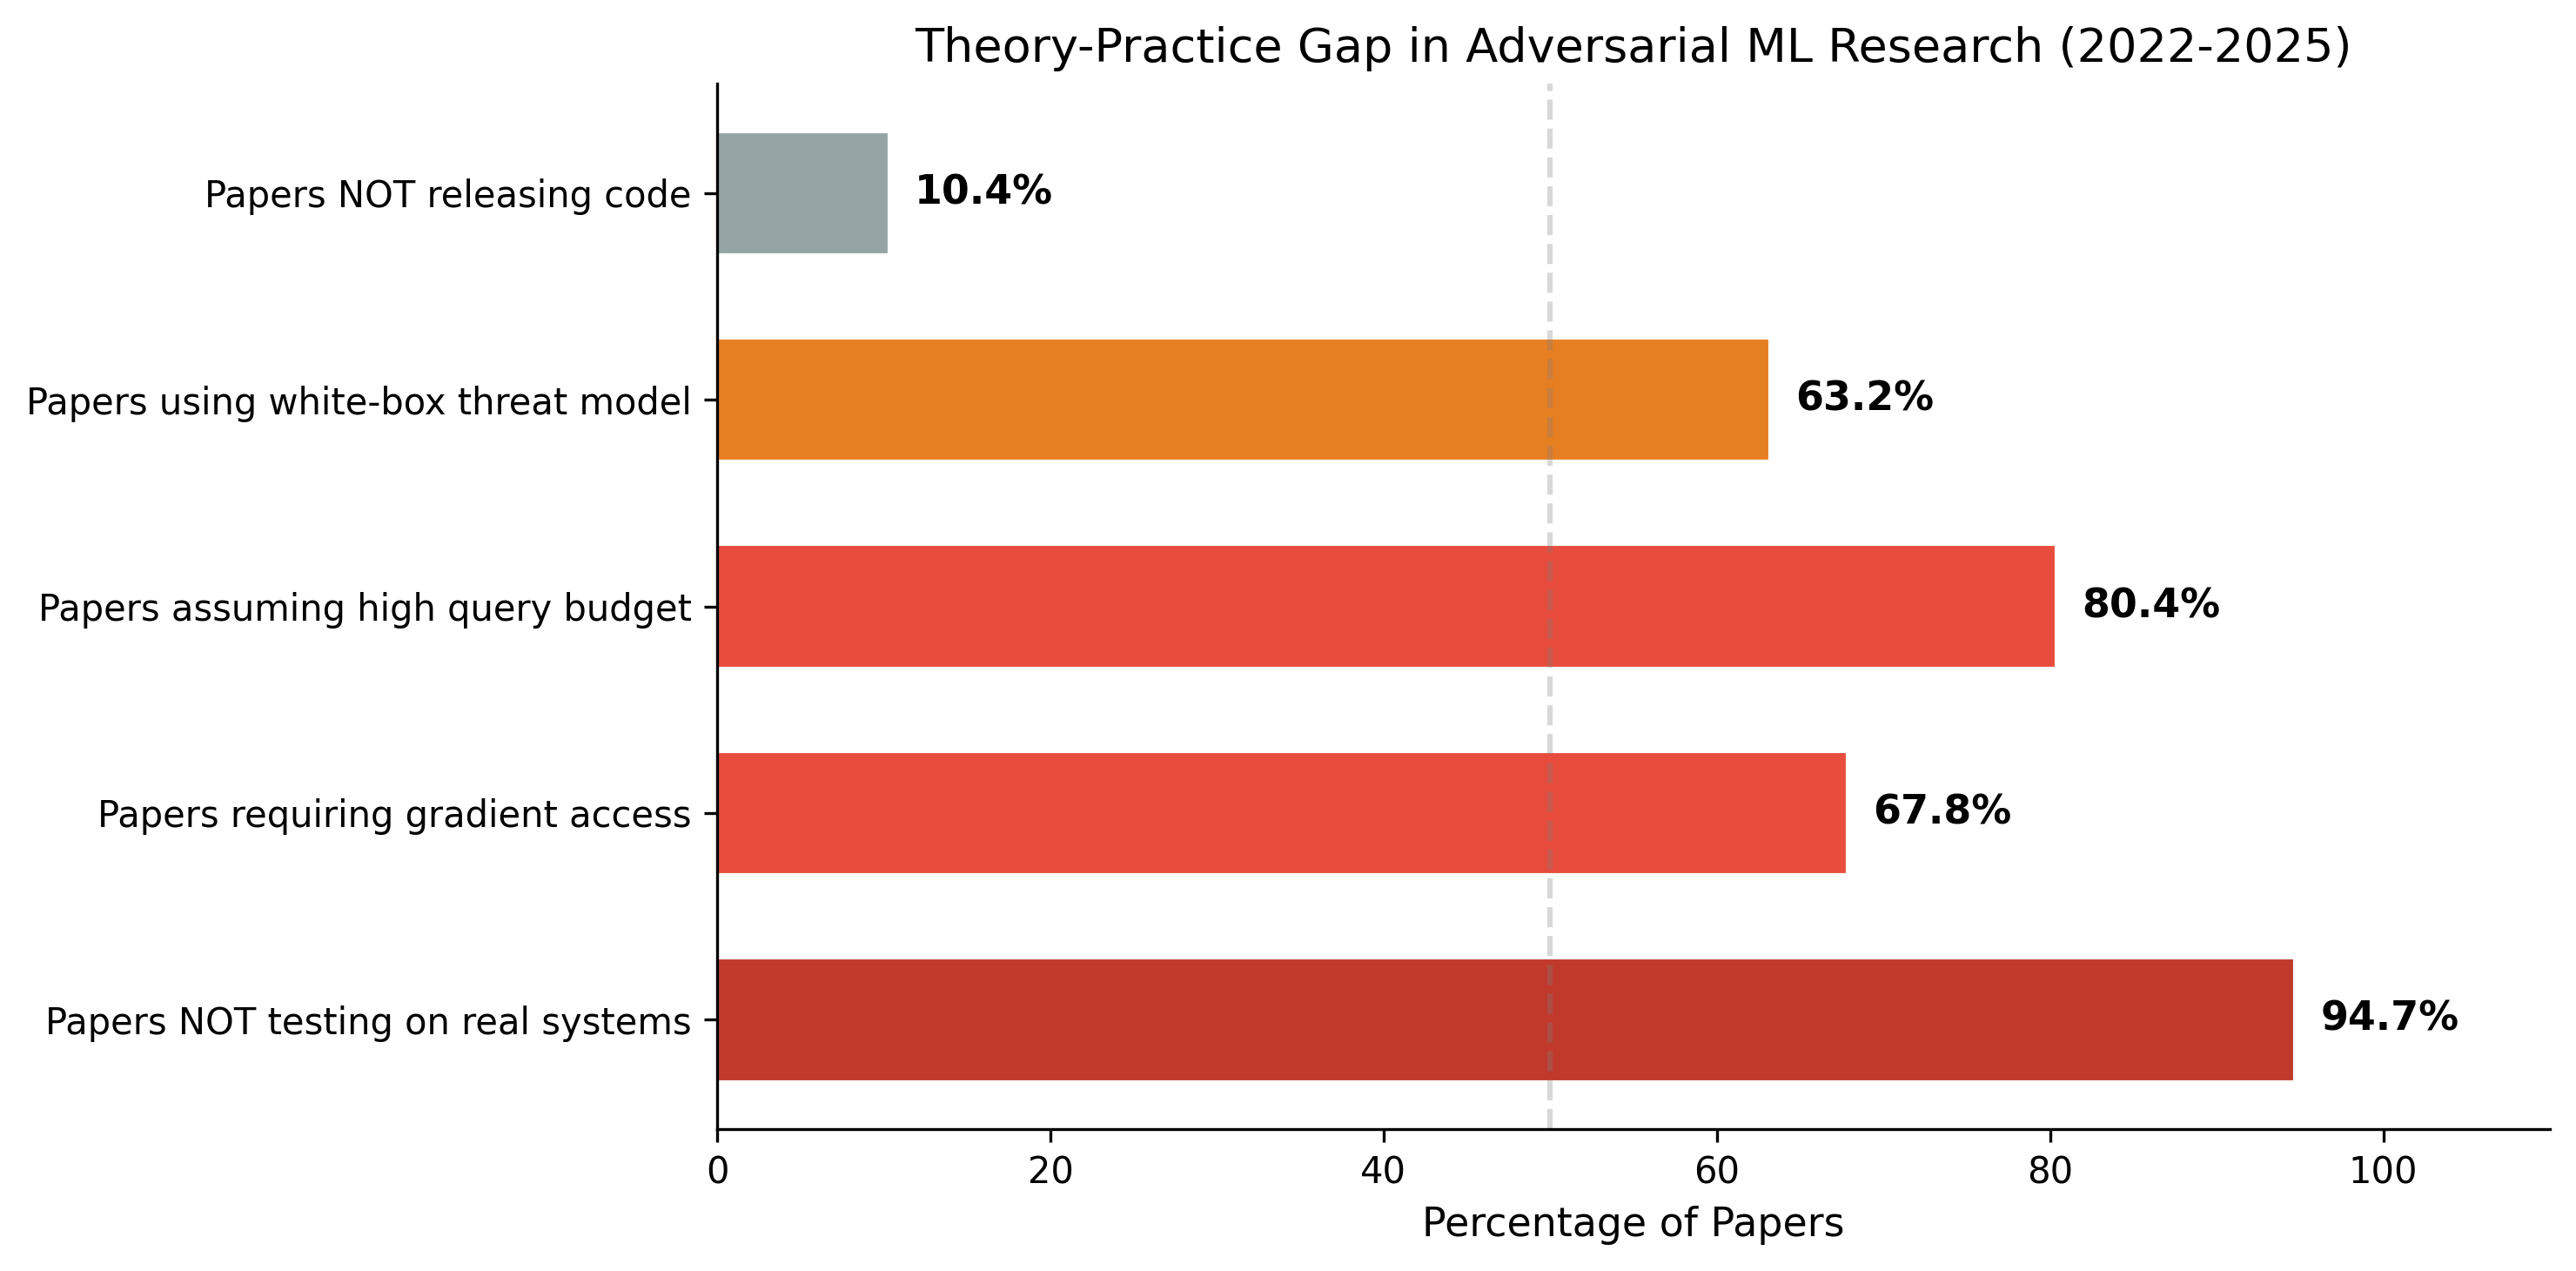
\includegraphics[width=\textwidth]{fig02_theory_practice_gap.png}
    \caption{Key indicators of the theory-practice gap across all 454 papers}
    \label{fig:gap_overview}
\end{figure}

\paragraph{Real-World Evaluation.}
Only \textbf{5.3\%} [95\% CI: 3.6\%, 7.6\%] of papers (24 of 454) included experiments on operational systems; the remainder relied on offline datasets, simulated environments, or research prototypes (Fig.~\ref{fig:real_world}). Papers that do test on real systems often reveal significant gaps between laboratory and field performance. Nayan et al.~\cite{nayan2024sok} found many academic model extraction attacks difficult to reproduce on actual services, and Layton et al.~\cite{layton2024sok} observed similar patterns for deepfake detection on realistic distributions.

\begin{figure}[htbp]
    \centering
    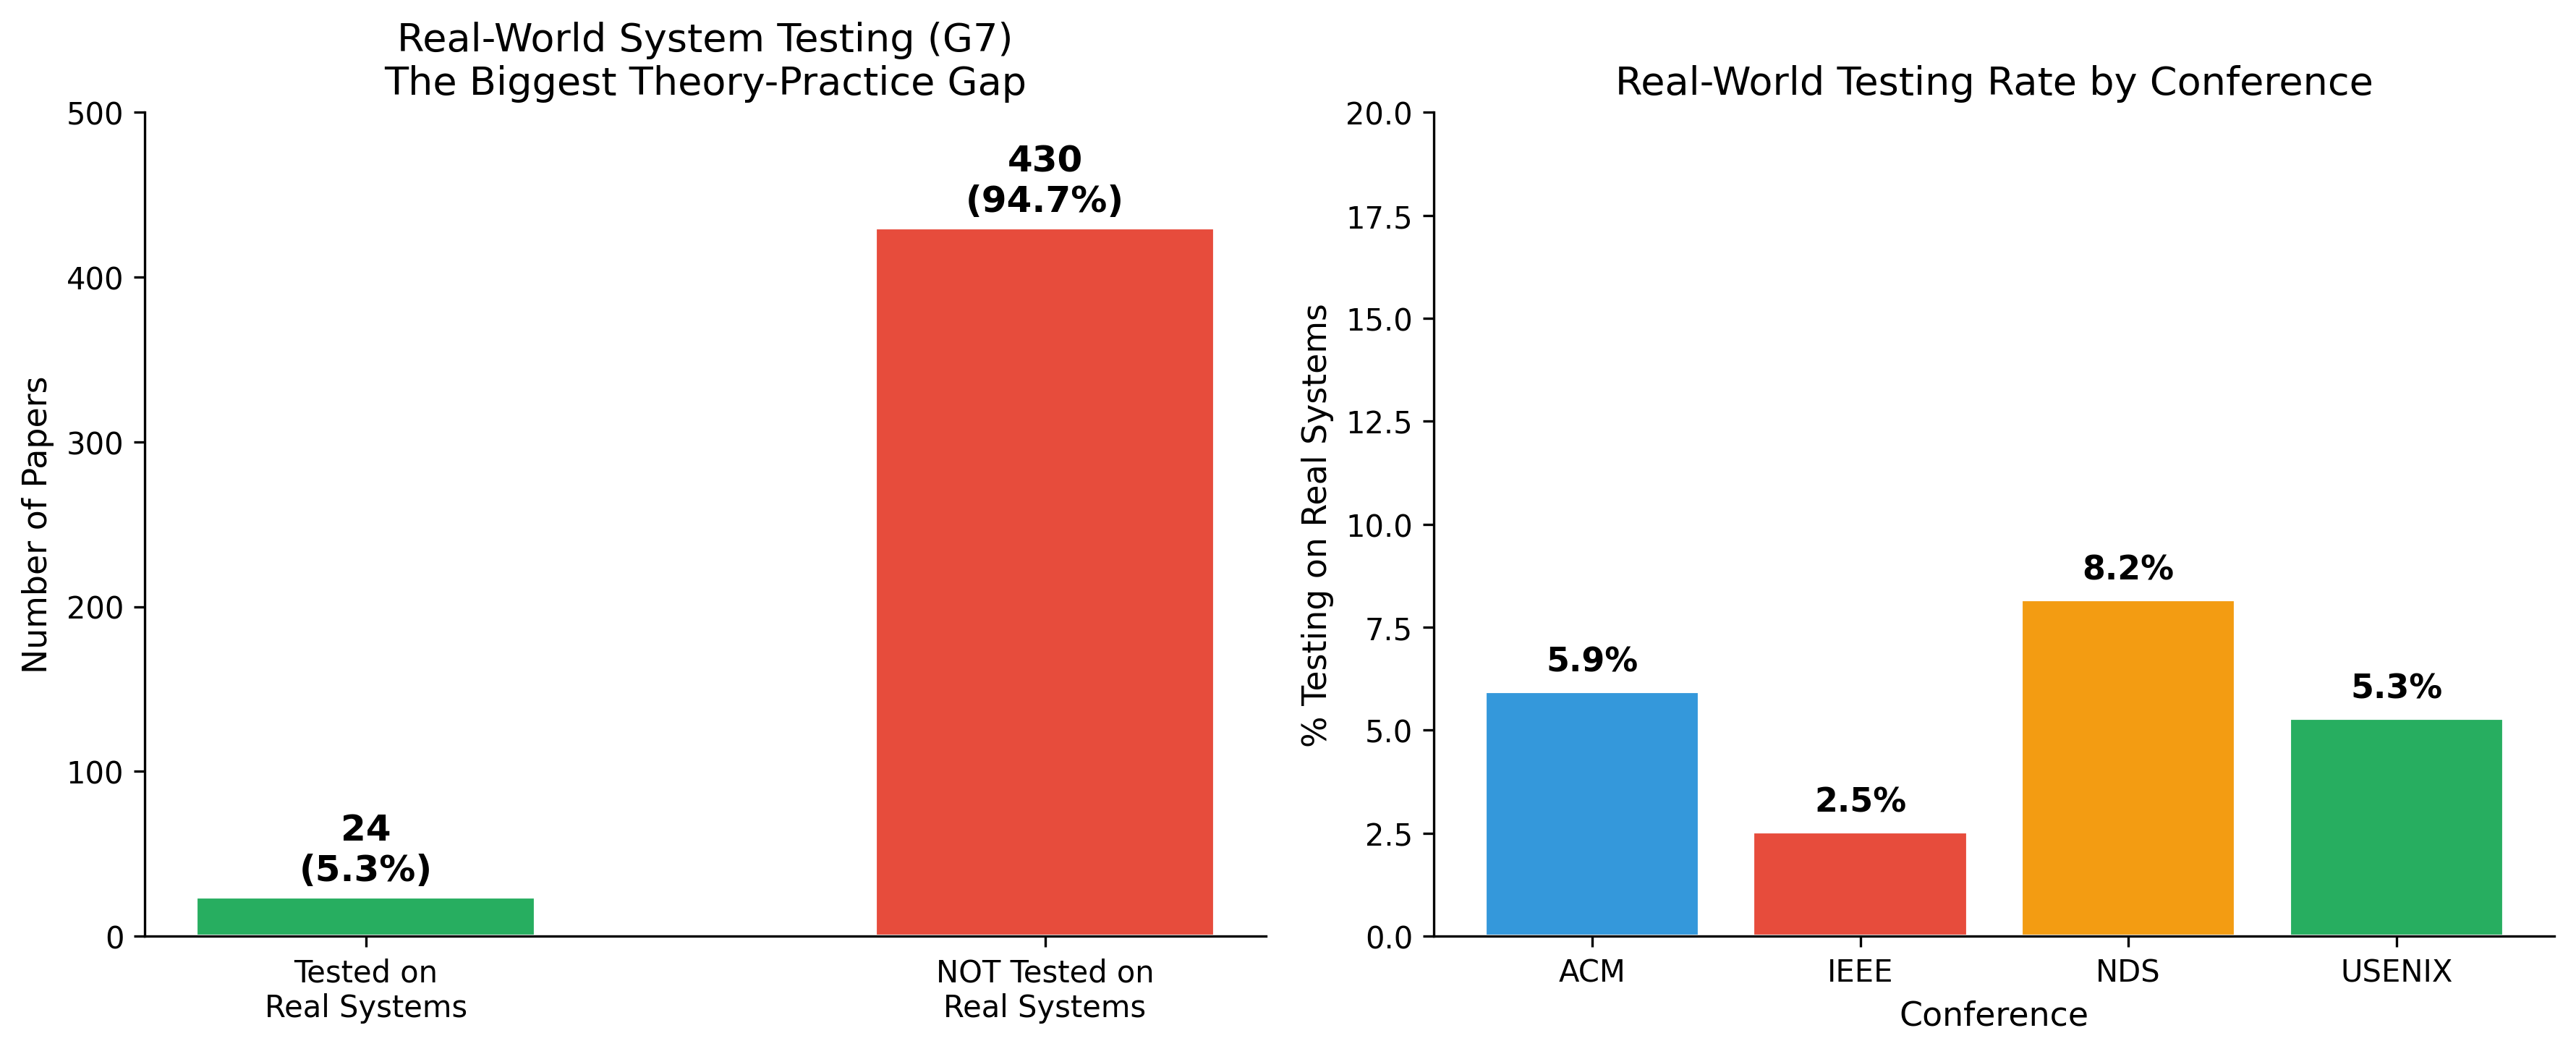
\includegraphics[width=\textwidth]{fig05_real_world_testing.png}
    \caption{Rate of real-world testing: only 5.3\% of papers evaluated on deployed systems.}
    \label{fig:real_world}
\end{figure}

\paragraph{Gradient Dependency.}
\textbf{67.8\%} [95\% CI: 63.4\%, 72.0\%] of papers require gradient information from target models, changing only modestly from 68.2\% in 2022 to 65.9\% in early 2025 (Fig.~\ref{fig:gradient}). Some recent work has embraced gradient-free approaches. For example, Eykholt et al.~\cite{eykholt2023uret} developed URET for domain-specific robustness evaluation, and LLM jailbreak attacks operate without gradients using natural language interaction~\cite{liu2024jailbreaking,yu2024jailbreak}. However, these remain exceptions.

\begin{figure}[htbp]
    \centering
    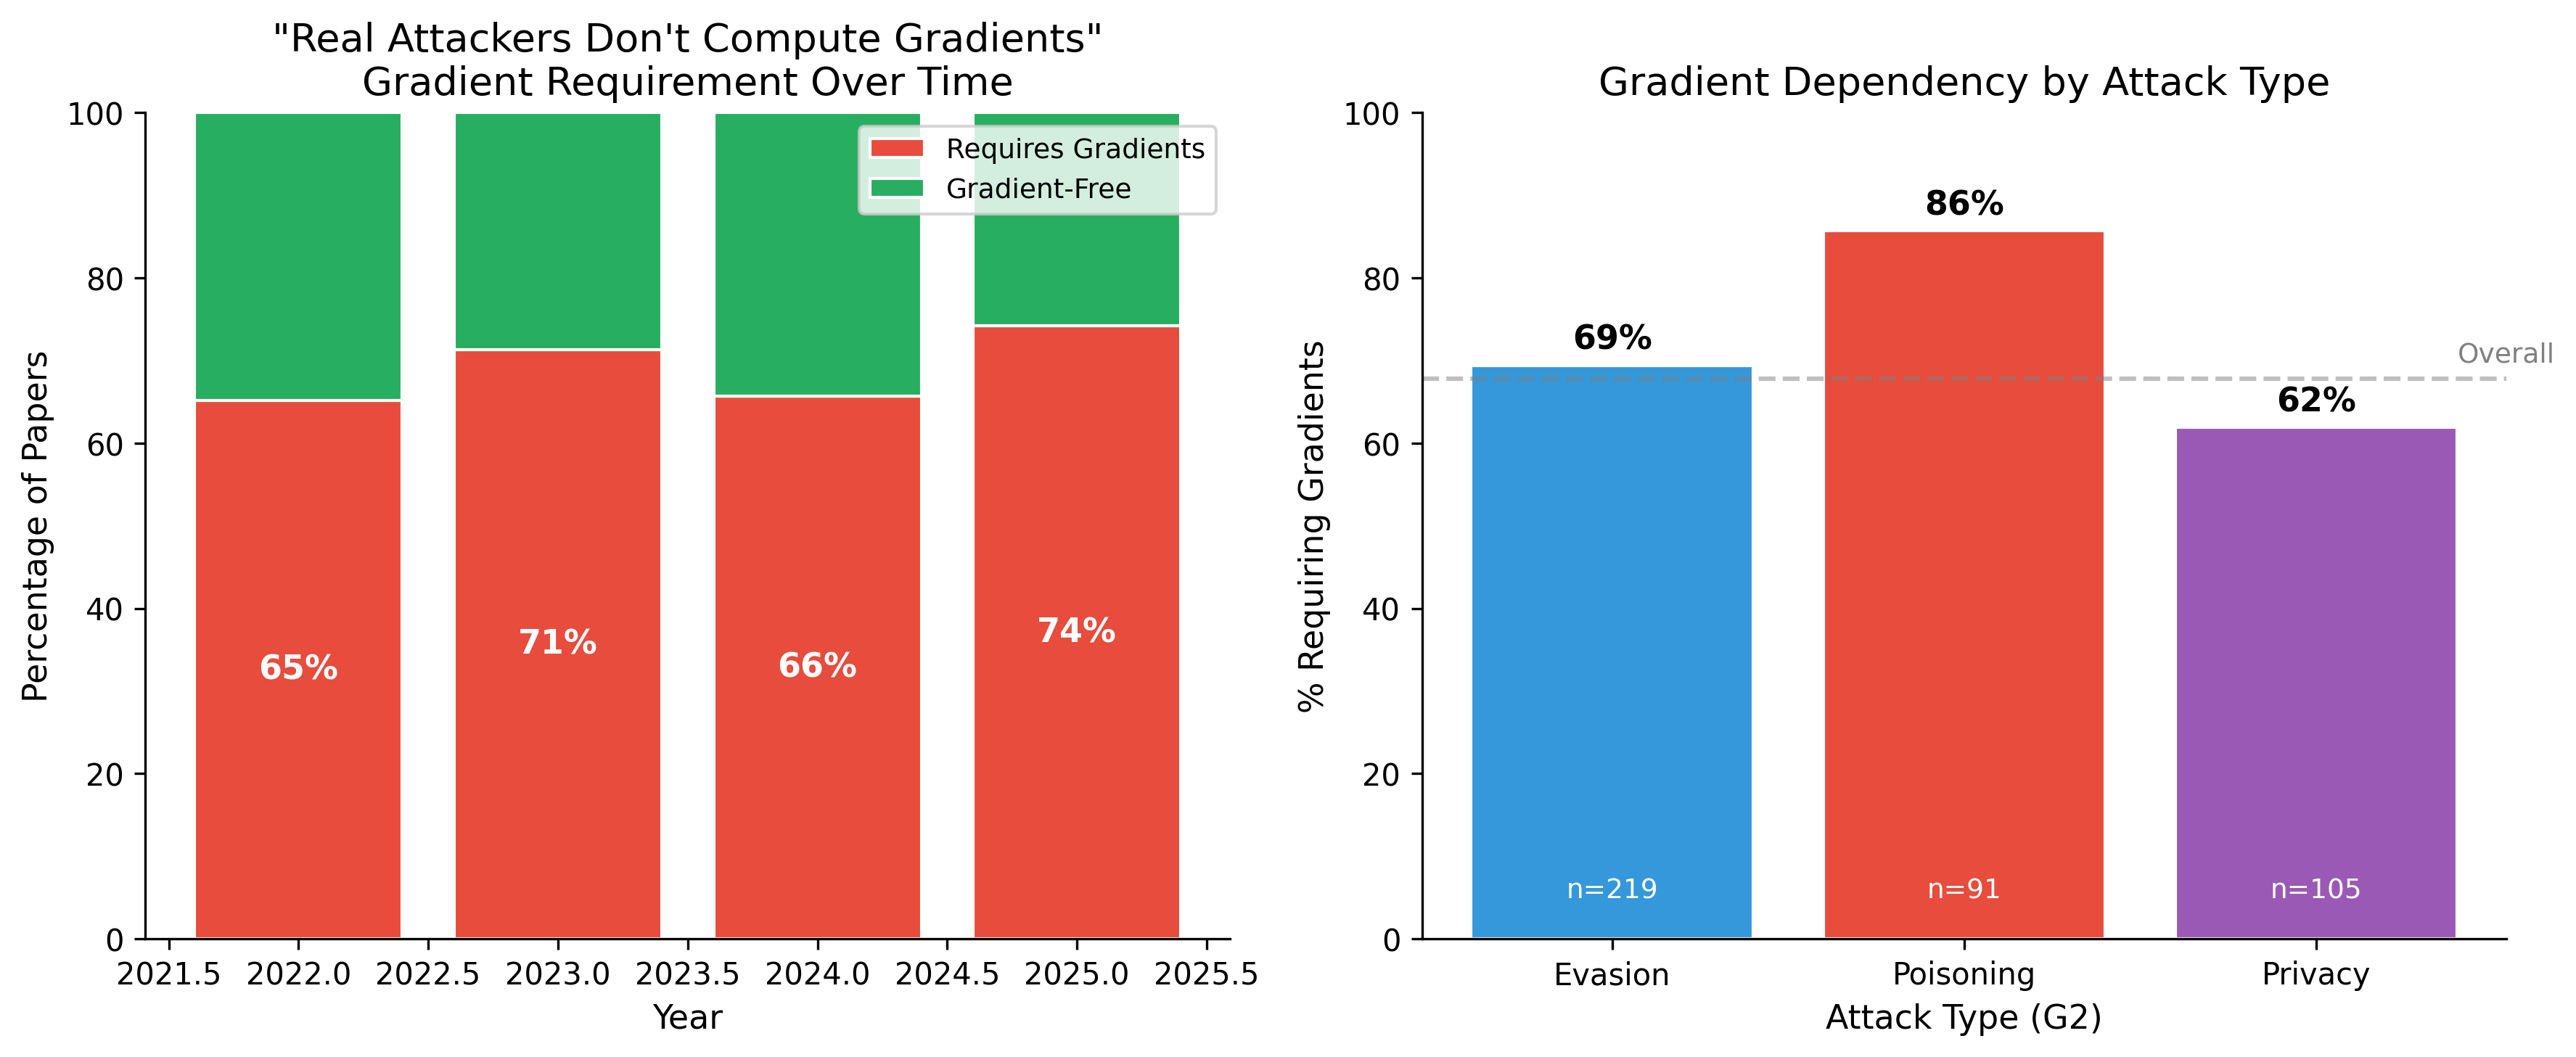
\includegraphics[width=\textwidth]{fig04_gradient_dependency.png}
    \caption{Gradient dependency over time: 67.8\% overall, with no meaningful reduction.}
    \label{fig:gradient}
\end{figure}

\paragraph{Threat Models and Query Budgets.}
\textbf{63.2\%} [95\% CI: 58.7\%, 67.5\%] of papers assume white-box adversaries; only 34.1\% consider black-box and 2.6\% gray-box scenarios (Fig.~\ref{fig:threat_model}). Among papers involving queries, \textbf{80.4\%} [95\% CI: 76.5\%, 83.8\%] assume budgets exceeding 1000 queries (Fig.~\ref{fig:query}), though notable exceptions exist: Tao et al.~\cite{tao2023hardbeat} achieved high attack success under hard-label constraints with few queries, and Wan et al.~\cite{wan2024bounceattack} developed a decision-based approach requiring minimal queries.

\begin{figure}[htbp]
    \centering
    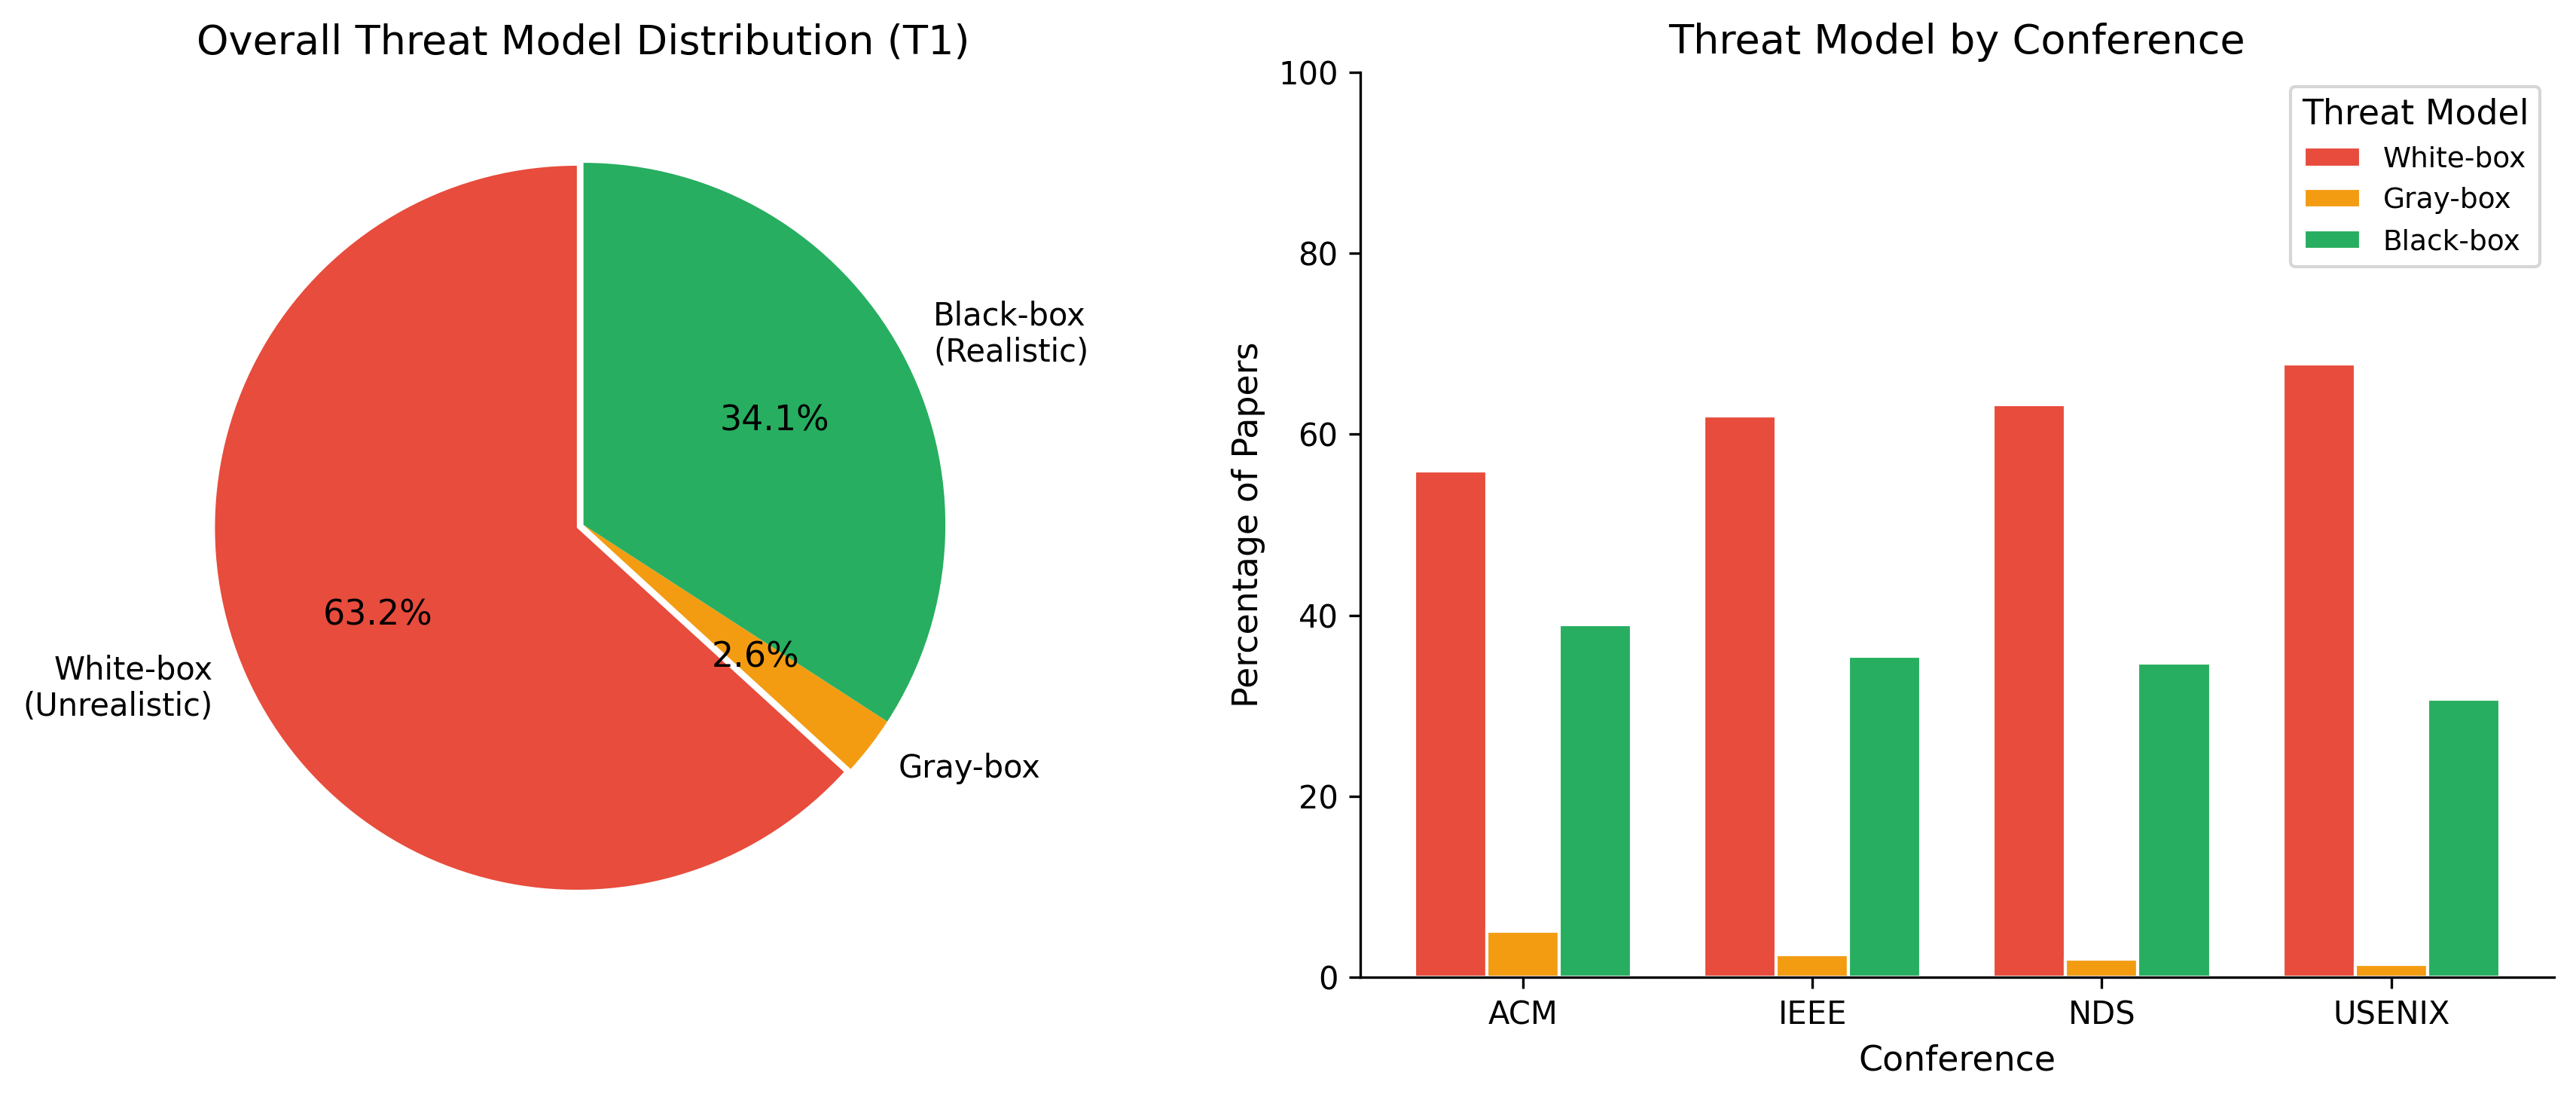
\includegraphics[width=\textwidth]{fig03_threat_model.png}
    \caption{Threat model assumptions: white-box scenarios dominate at 63.2\%.}
    \label{fig:threat_model}
\end{figure}

\begin{figure}[htbp]
    \centering
    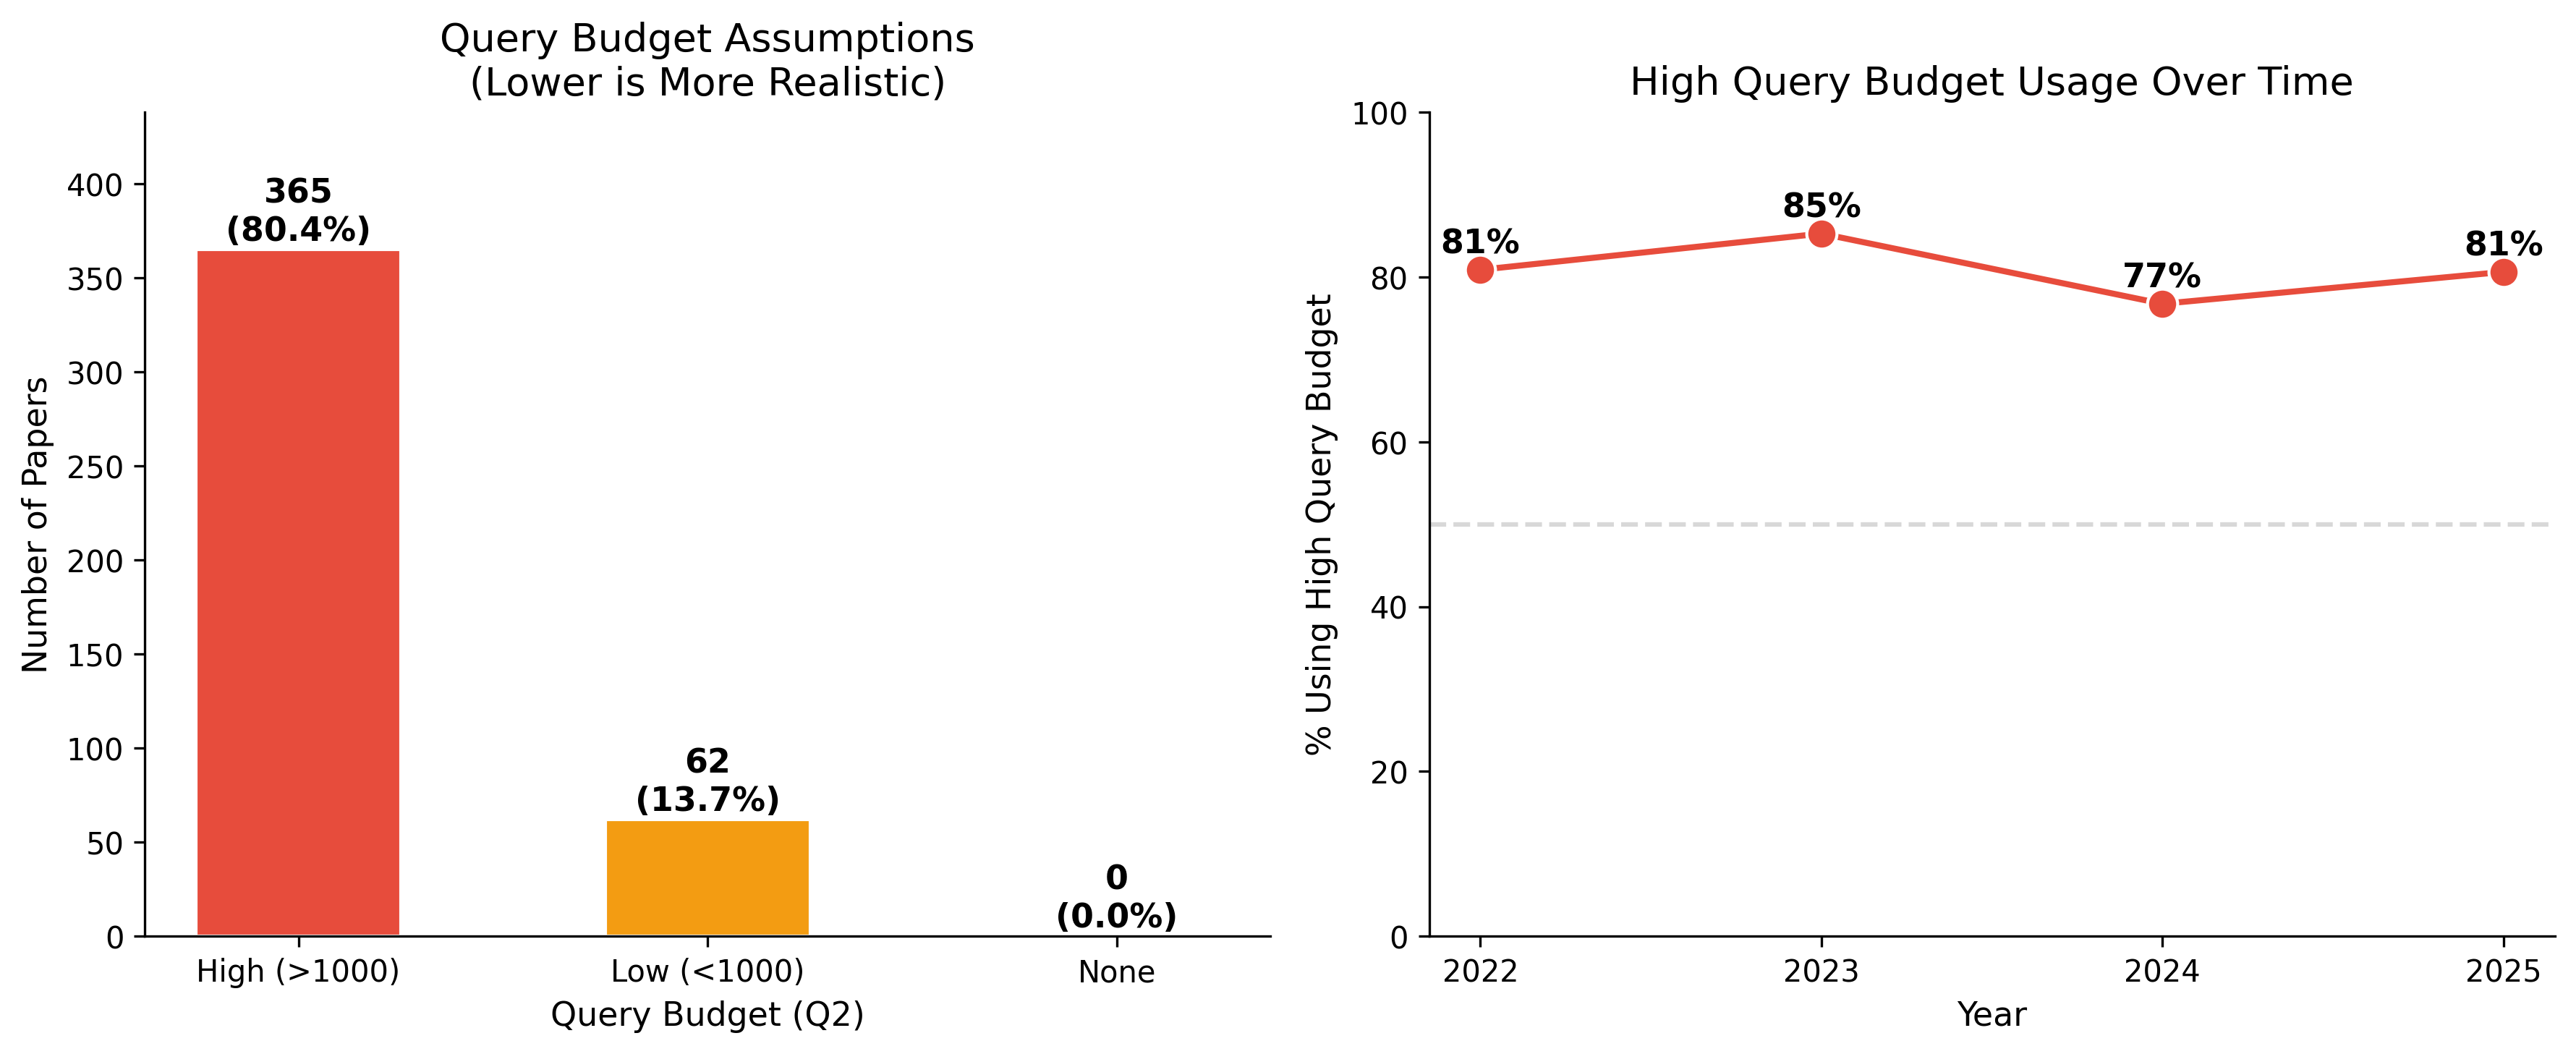
\includegraphics[width=\textwidth]{fig06_query_budget.png}
    \caption{Over 80\% of relevant papers assumed high query budgets ($>$1000).}
    \label{fig:query}
\end{figure}

\paragraph{Domain Bias and Gap Score.}
Approximately \textbf{65\%} of papers focus on image-based tasks, with text (11\%), audio (7\%), malware (6\%), and other domains (12\%) comprising the remainder (Fig.~\ref{fig:domains}). Per-domain analysis reveals substantial variation in practical alignment. Image-focused research exhibits the highest Gap Score (3.57), with 83.3\% requiring gradients and only 1.7\% testing on real systems. In contrast, text/LLM research shows a Gap Score of 2.62 (43.8\% gradient dependency), audio research 1.83 (26.7\% gradients, 36.7\% real-system testing), and malware research 2.41 (37.0\% gradients). This suggests that the overall gap is driven primarily by vision-centric research, while emerging domains like LLMs demonstrate greater practical alignment. The average Gap Score across all papers was \textbf{3.17 out of 6}, with 15.0\% [95\% CI: 12.0\%, 18.6\%] scoring 0 to 1 (Fig.~\ref{fig:gap_score}). Cross-venue variation was minimal and not statistically significant (p = 0.20 to 0.65): CCS averaged 3.04, NDSS 3.12, S\&P 3.18, and USENIX 3.25.

\begin{figure}[htbp]
    \centering
    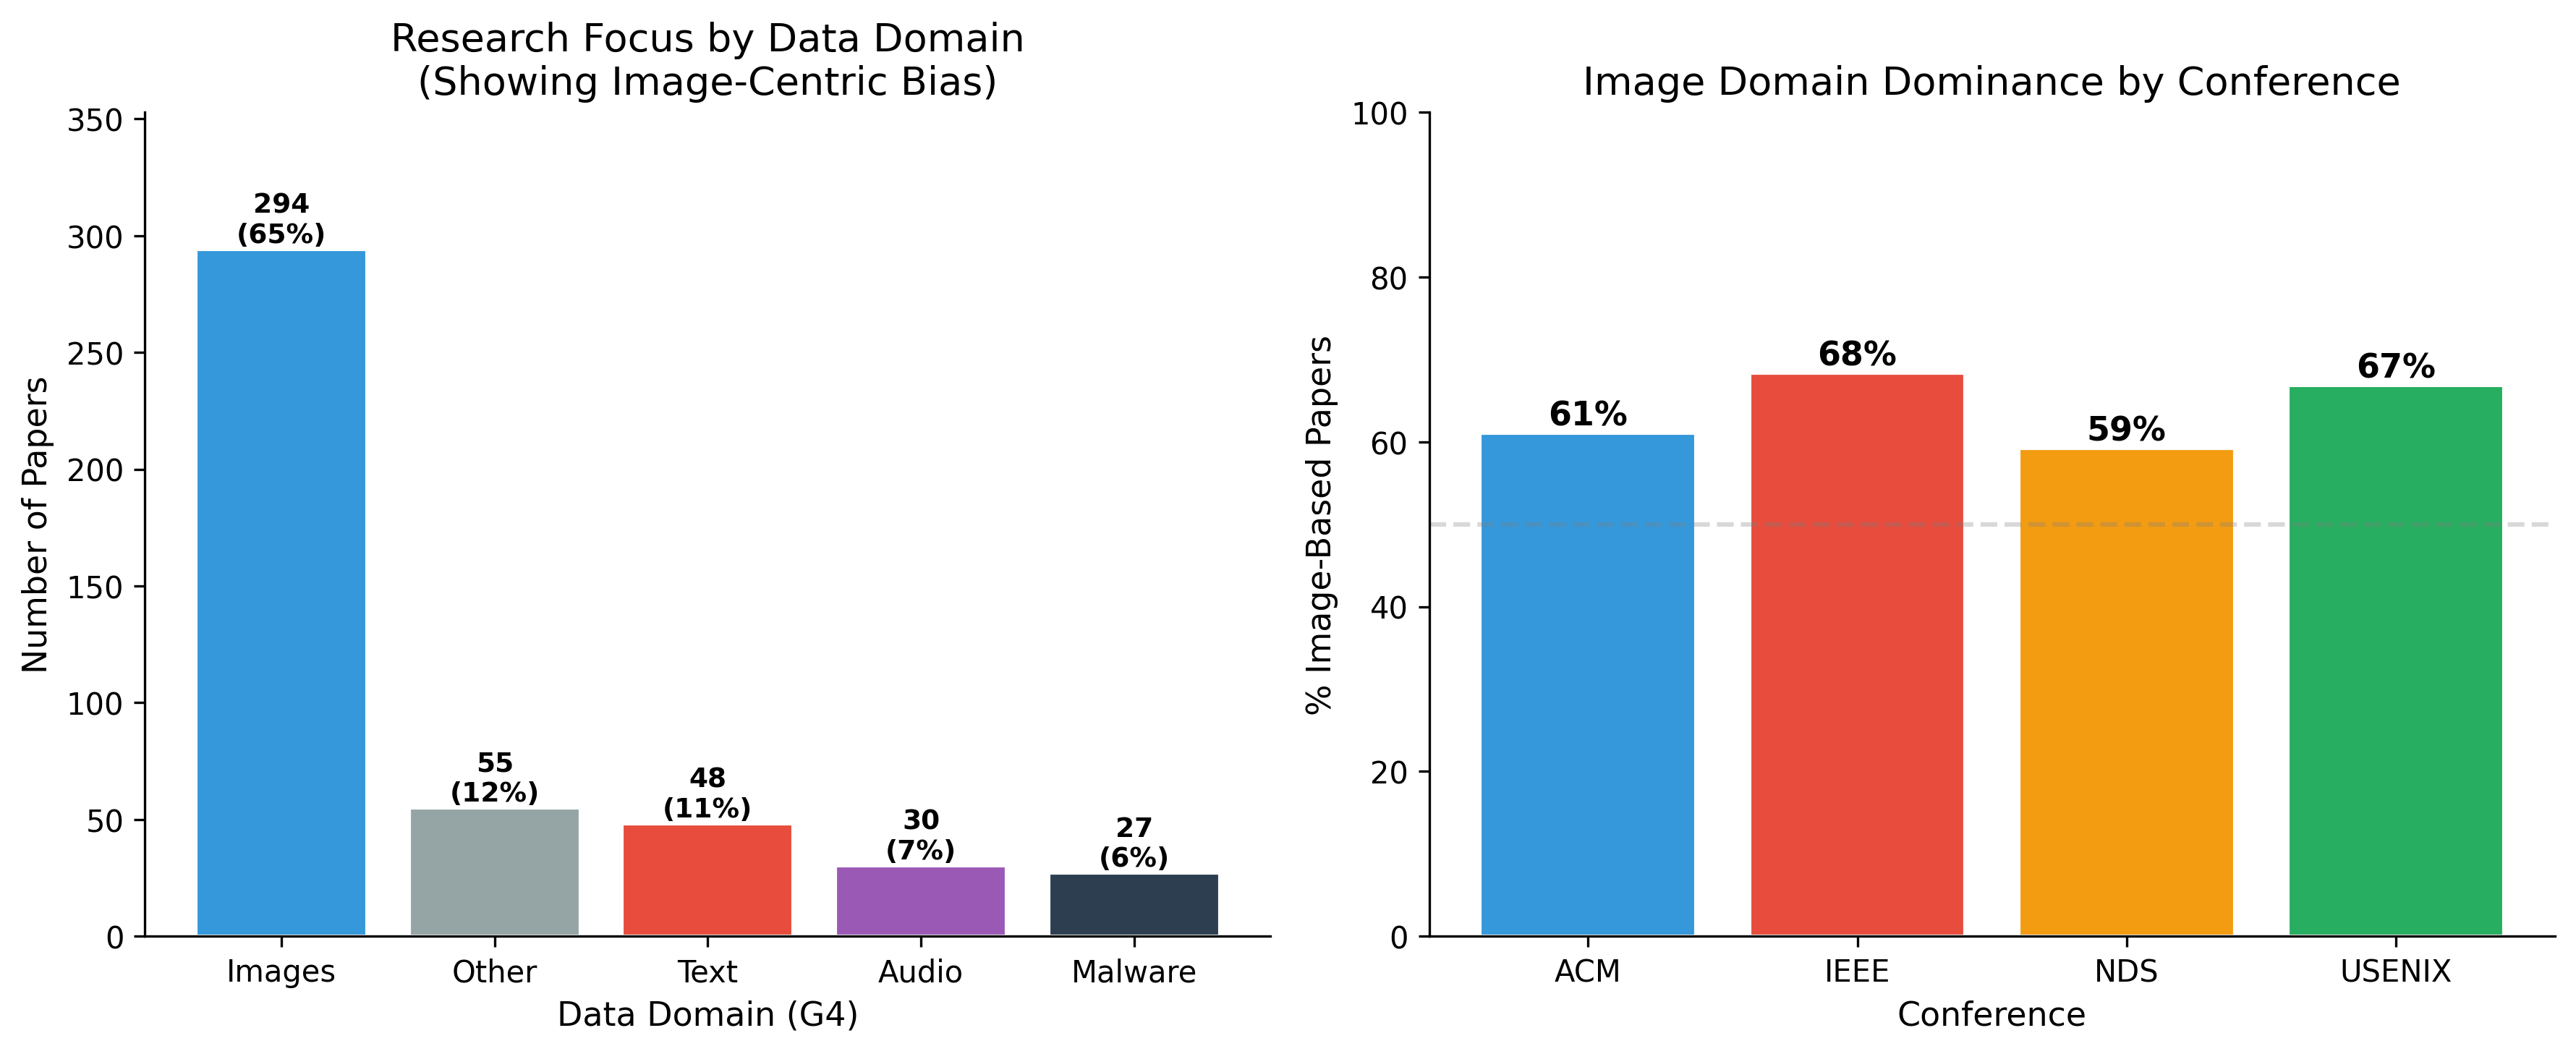
\includegraphics[width=\textwidth]{fig08_data_domains.png}
    \caption{Data domain distribution: image-focused research dominates at 65\%.}
    \label{fig:domains}
\end{figure}

\begin{figure}[htbp]
    \centering
    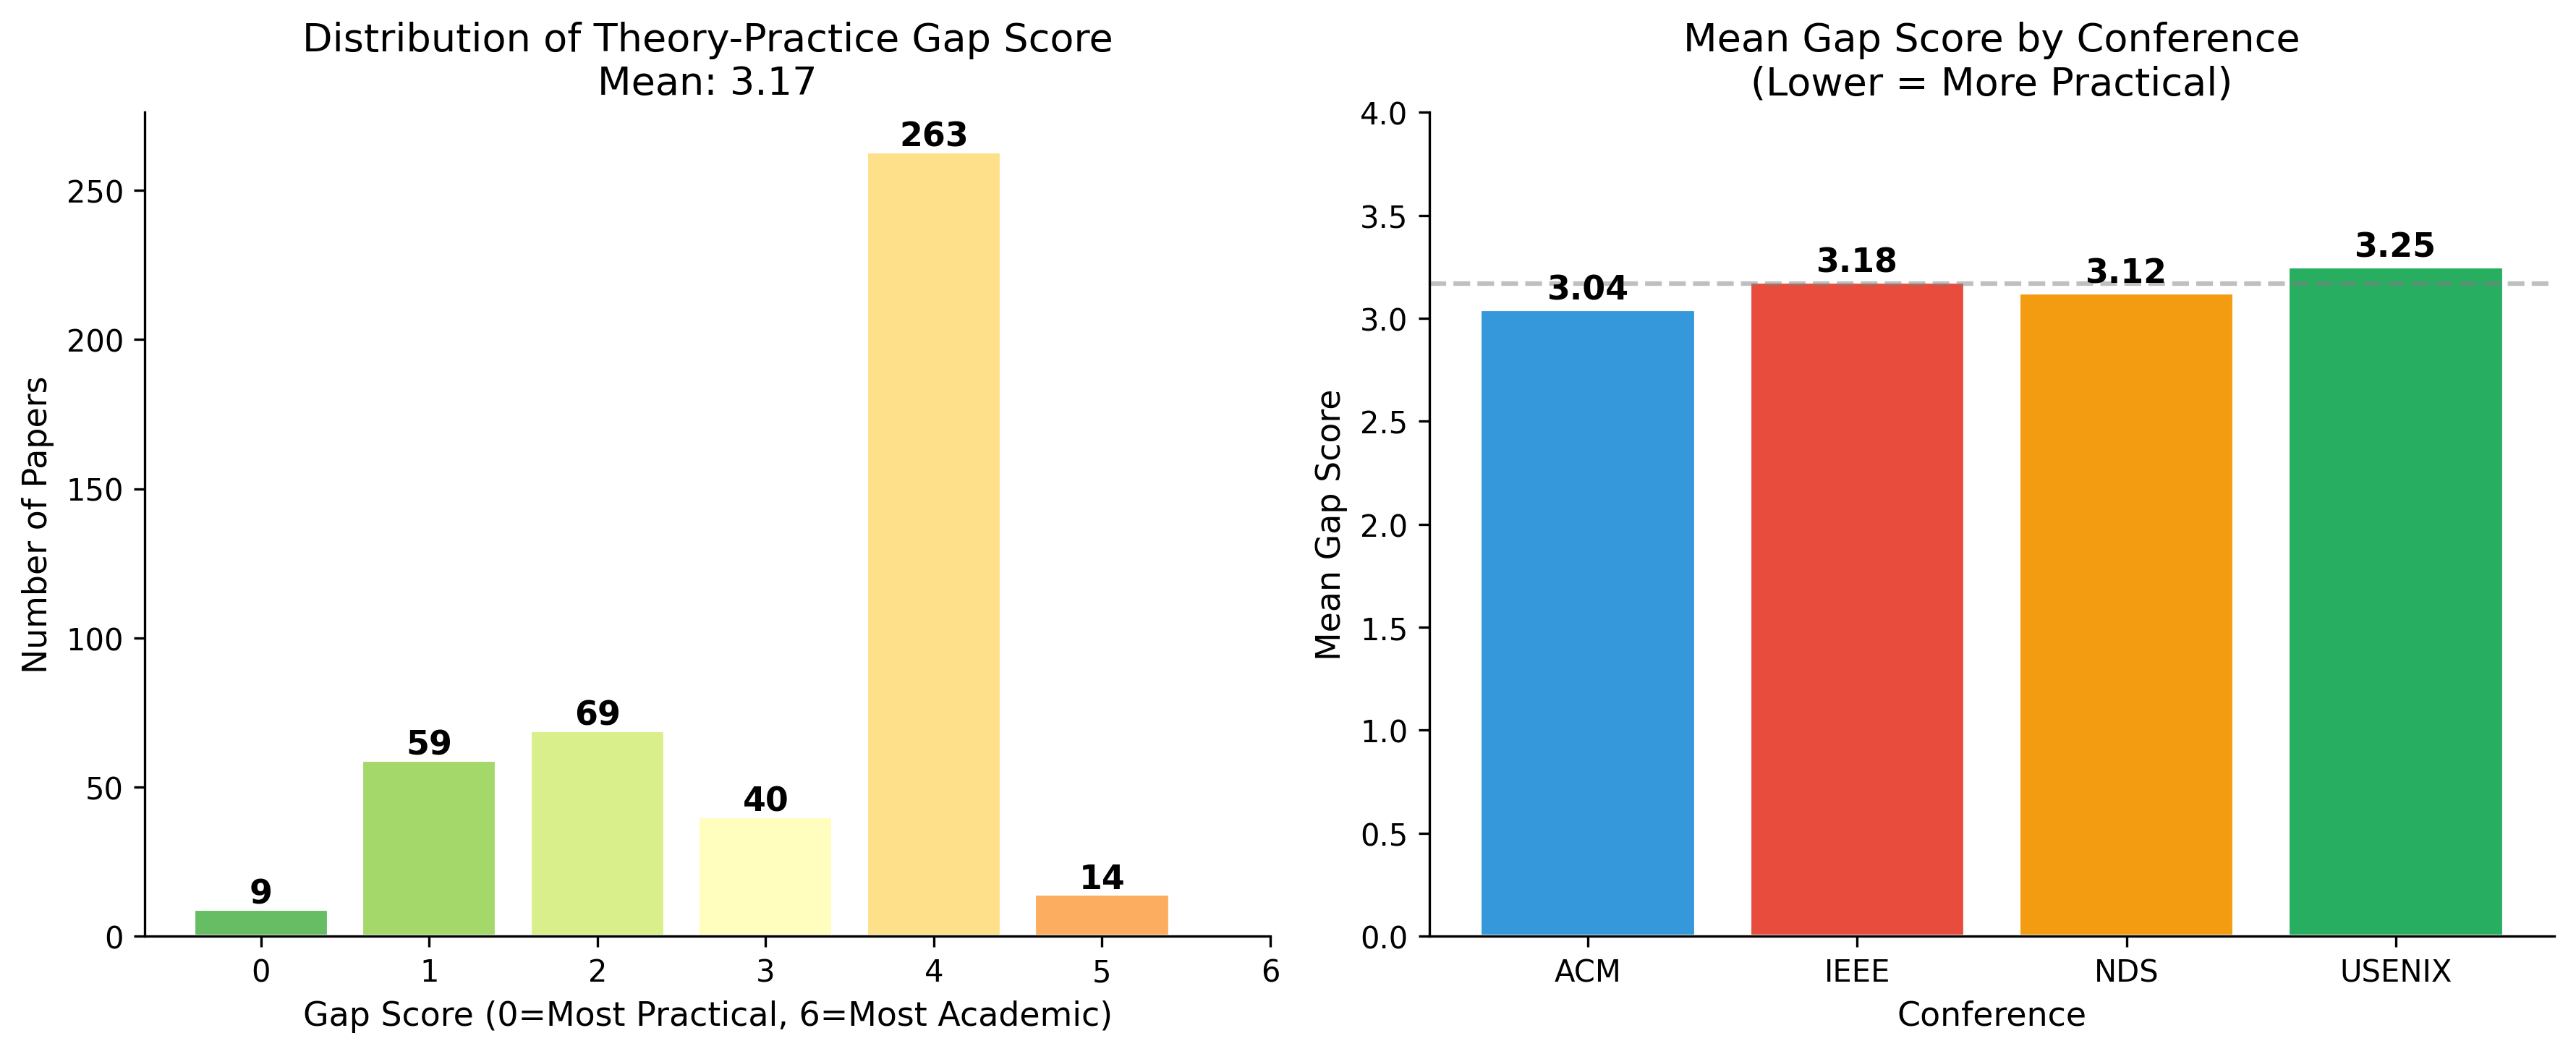
\includegraphics[width=\textwidth]{fig12_gap_score.png}
    \caption{Gap Score distribution: the typical paper incorporates about half of the tracked impractical assumptions.}
    \label{fig:gap_score}
\end{figure}

\paragraph{Research Patterns.}
Beyond these statistics, three patterns emerge. First, defenses often trade robustness for accuracy, latency, or usability~\cite{xiang2022patchcleanser,ahmed2022keyword,liu2022mldoctor}, though recent work reports reduced utility costs~\cite{li2024mist,wang2025camp}. Second, research increasingly addresses physical and system-level contexts including autonomous driving~\cite{jia2022physical}, production ML pipelines~\cite{nasr2025magika}, and LLM jailbreaking~\cite{chao2023jailbreaking}. Third, only a small subset addresses economic incentives or organizational factors~\cite{mink2023barriers}.

%==============================================================================
\section{Why This Gap Matters: Foundation Models and Emerging Threats}
\label{sec:foundation}

The proliferation of large language models and multimodal foundation models has introduced adversarial challenges that make the theory-practice gap more consequential. These systems process discrete tokens, accept multimodal inputs, operate through rate-limited APIs, and increasingly control real-world actions through agentic workflows. LLM jailbreaking research exhibits the same gap patterns: automated methods like GCG~\cite{zou2023universal} require white-box gradient access, while practical attacks like PAIR~\cite{chao2023jailbreaking} and TAP~\cite{mehrotra2024tree} succeed with approximately 20 queries using black-box LLM-based refinement. Prompt injection attacks~\cite{liu2024prompt,greshake2023youve} manipulate model behavior through malicious instructions in retrieved content, exploiting system integration rather than model internals. Vision-language models introduce cross-modal attack surfaces where adversarial images trigger harmful text generation~\cite{qi2024visual} and encoded text bypasses filters~\cite{gong2024figstep}, while agentic systems with tool access face amplified risks from indirect prompt injection~\cite{zhan2024injecagent}.

Real-world incidents demonstrate these threats. In November 2025, Anthropic disclosed a state-sponsored campaign where an AI agent autonomously conducted reconnaissance, exploit generation, and data exfiltration against approximately thirty targets~\cite{anthropic2025ai}, performing 80 to 90\% of operational workload (Fig.~\ref{fig:claude}). The attack exploited agentic execution and jailbreaking, not gradient access. Similarly, EchoLeak exfiltrated data from Microsoft 365 Copilot through malicious documents~\cite{aim2025echoleak}, and training data extraction from ChatGPT succeeded through structured prompts at modest cost~\cite{nasr2023scalable}. Foundation models pose systemic risks because vulnerabilities in widely-deployed base models propagate across downstream applications. The most effective automated attacks require white-box access or substantial queries, yet commercial APIs provide only black-box access with rate limits. Deployed models receive frequent updates, invalidating discovered vulnerabilities. These characteristics amplify the consequences of the theory-practice gap, as academic research optimizes for threat models that rarely materialize while operational threats exploit system integration, multimodal capabilities, and automation workflows that academic work largely ignores.

\begin{figure}[!htb]
    \centering
    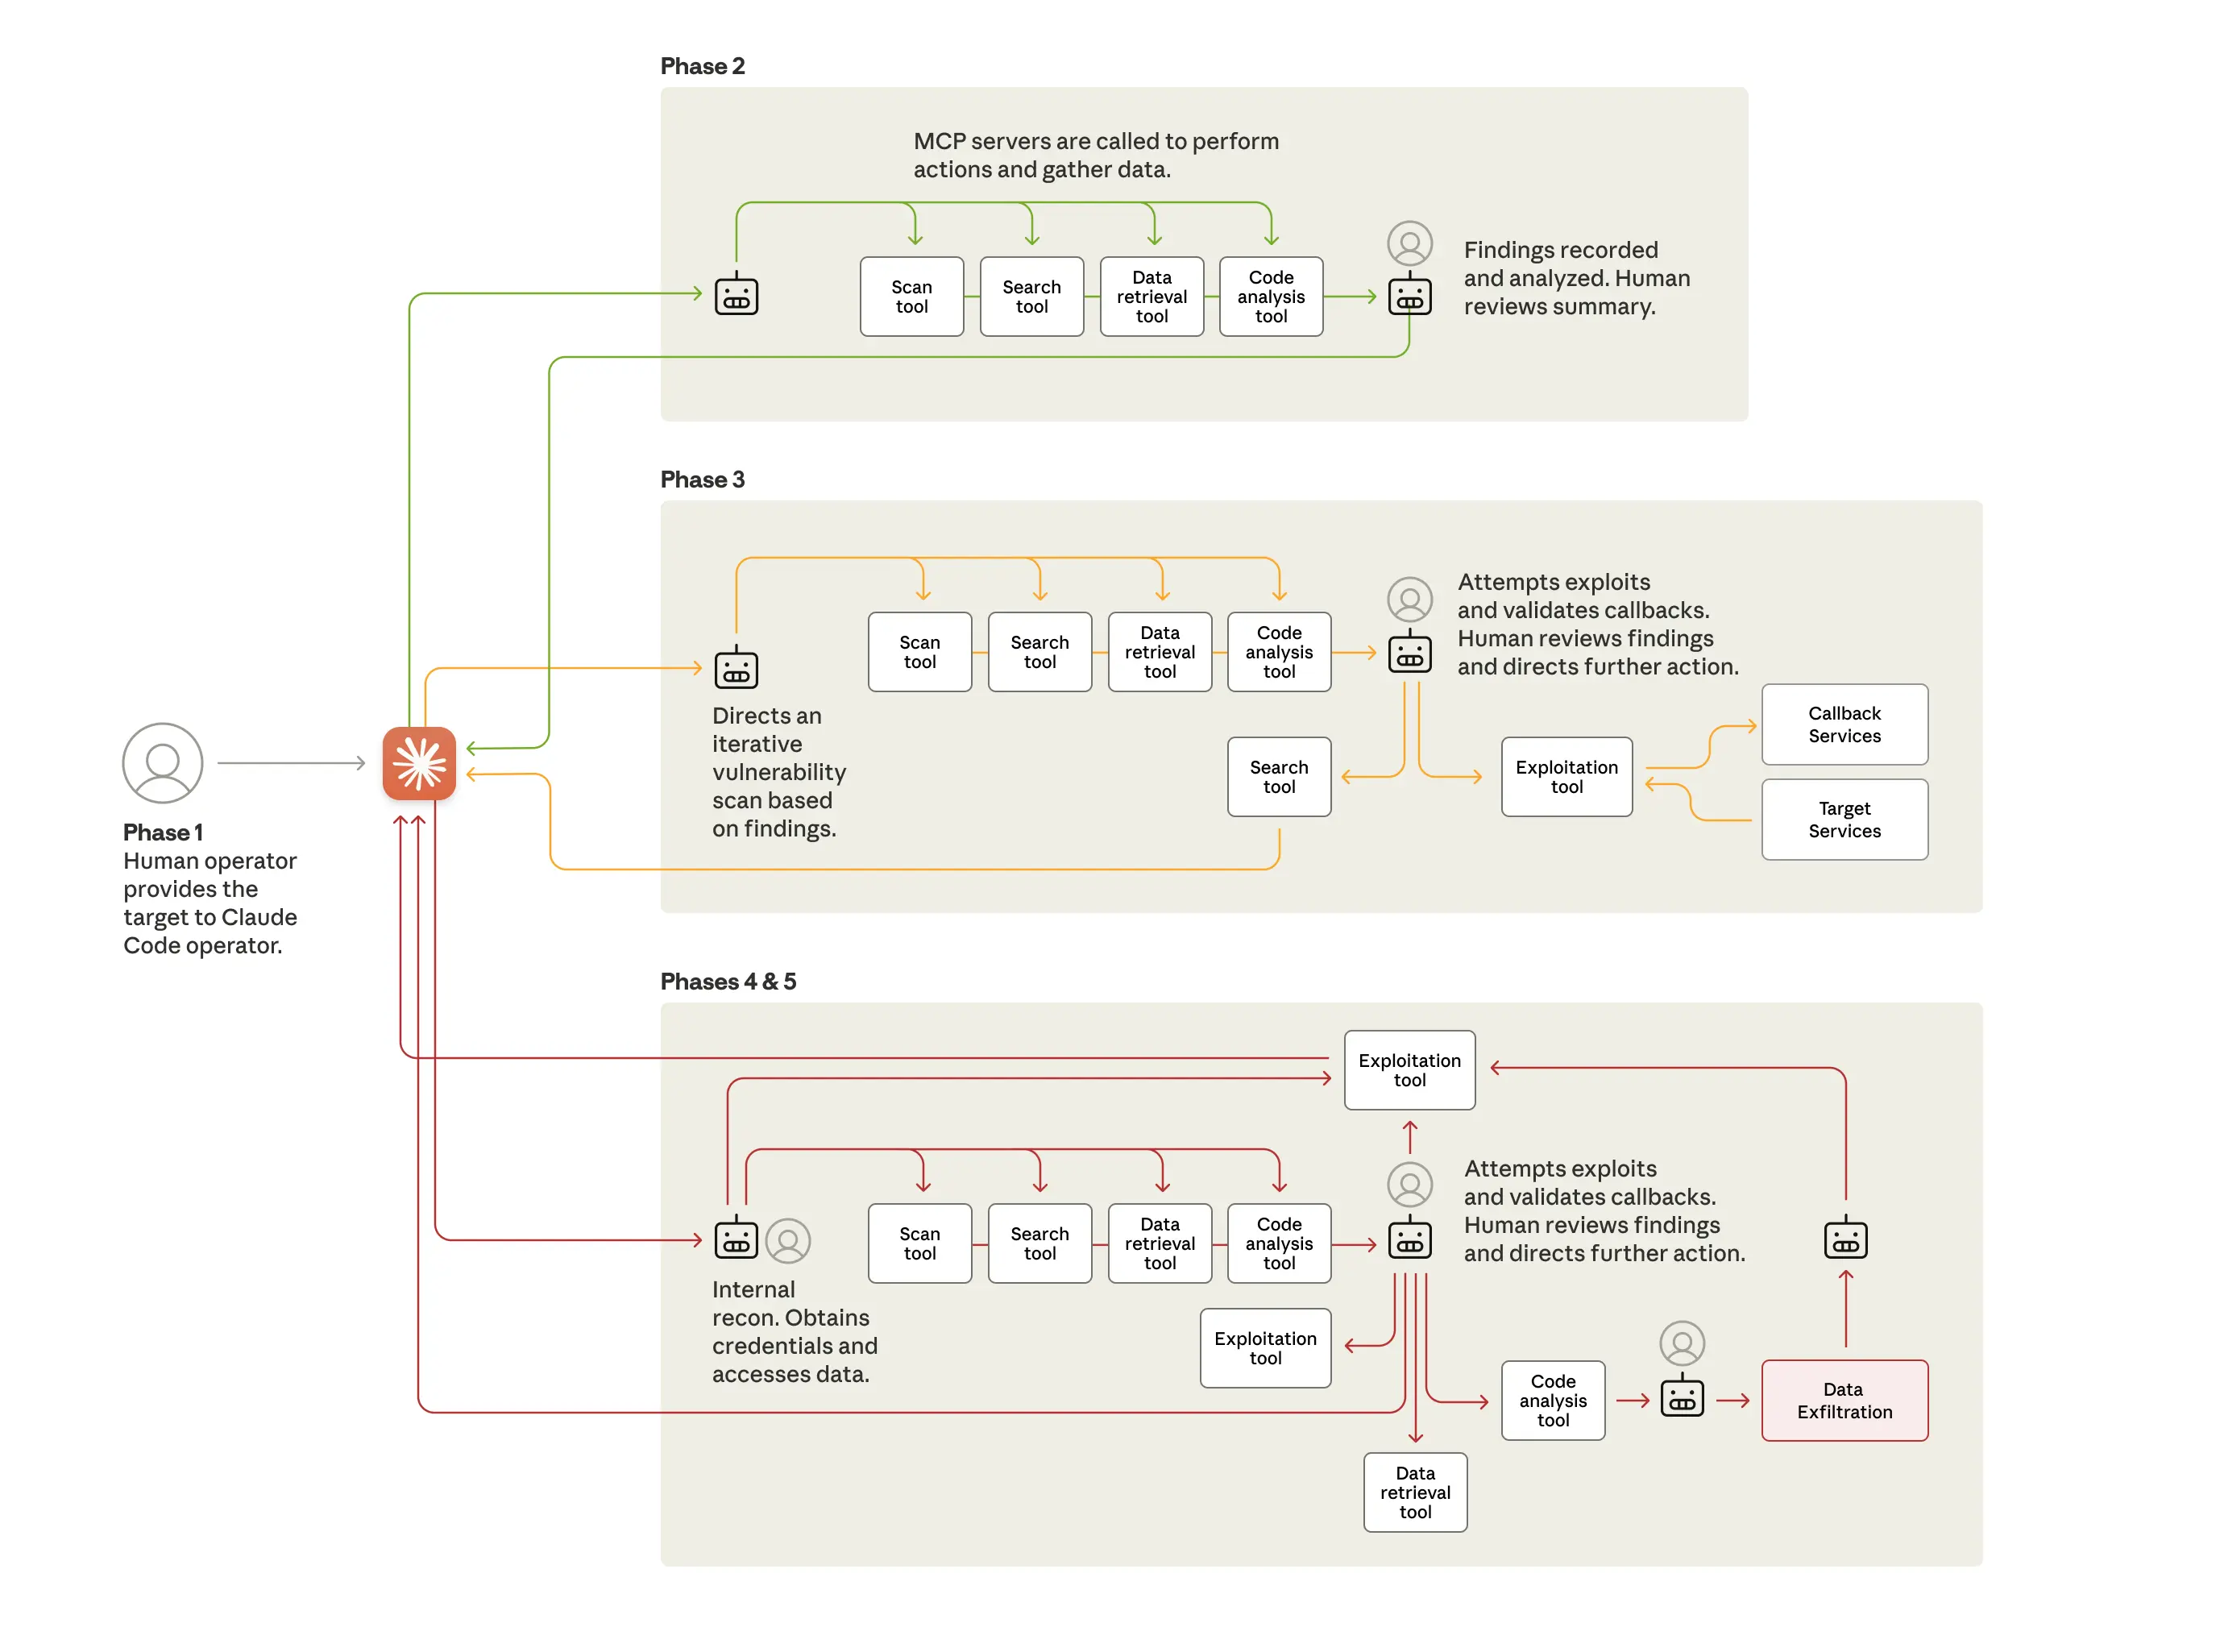
\includegraphics[width=\textwidth]{claude.png}
    \caption{The lifecycle of an AI-orchestrated cyberattack, showing human-led targeting transitioning to largely AI-driven execution~\cite{anthropic2025ai}}
    \label{fig:claude}
\end{figure}

\clearpage
%==============================================================================
\section{Temporal Trends}
\label{sec:trends}

Figure~\ref{fig:trends} summarizes how indicators evolved following the Apruzzese et al.\ critique.

\begin{figure}[htbp]
    \centering
    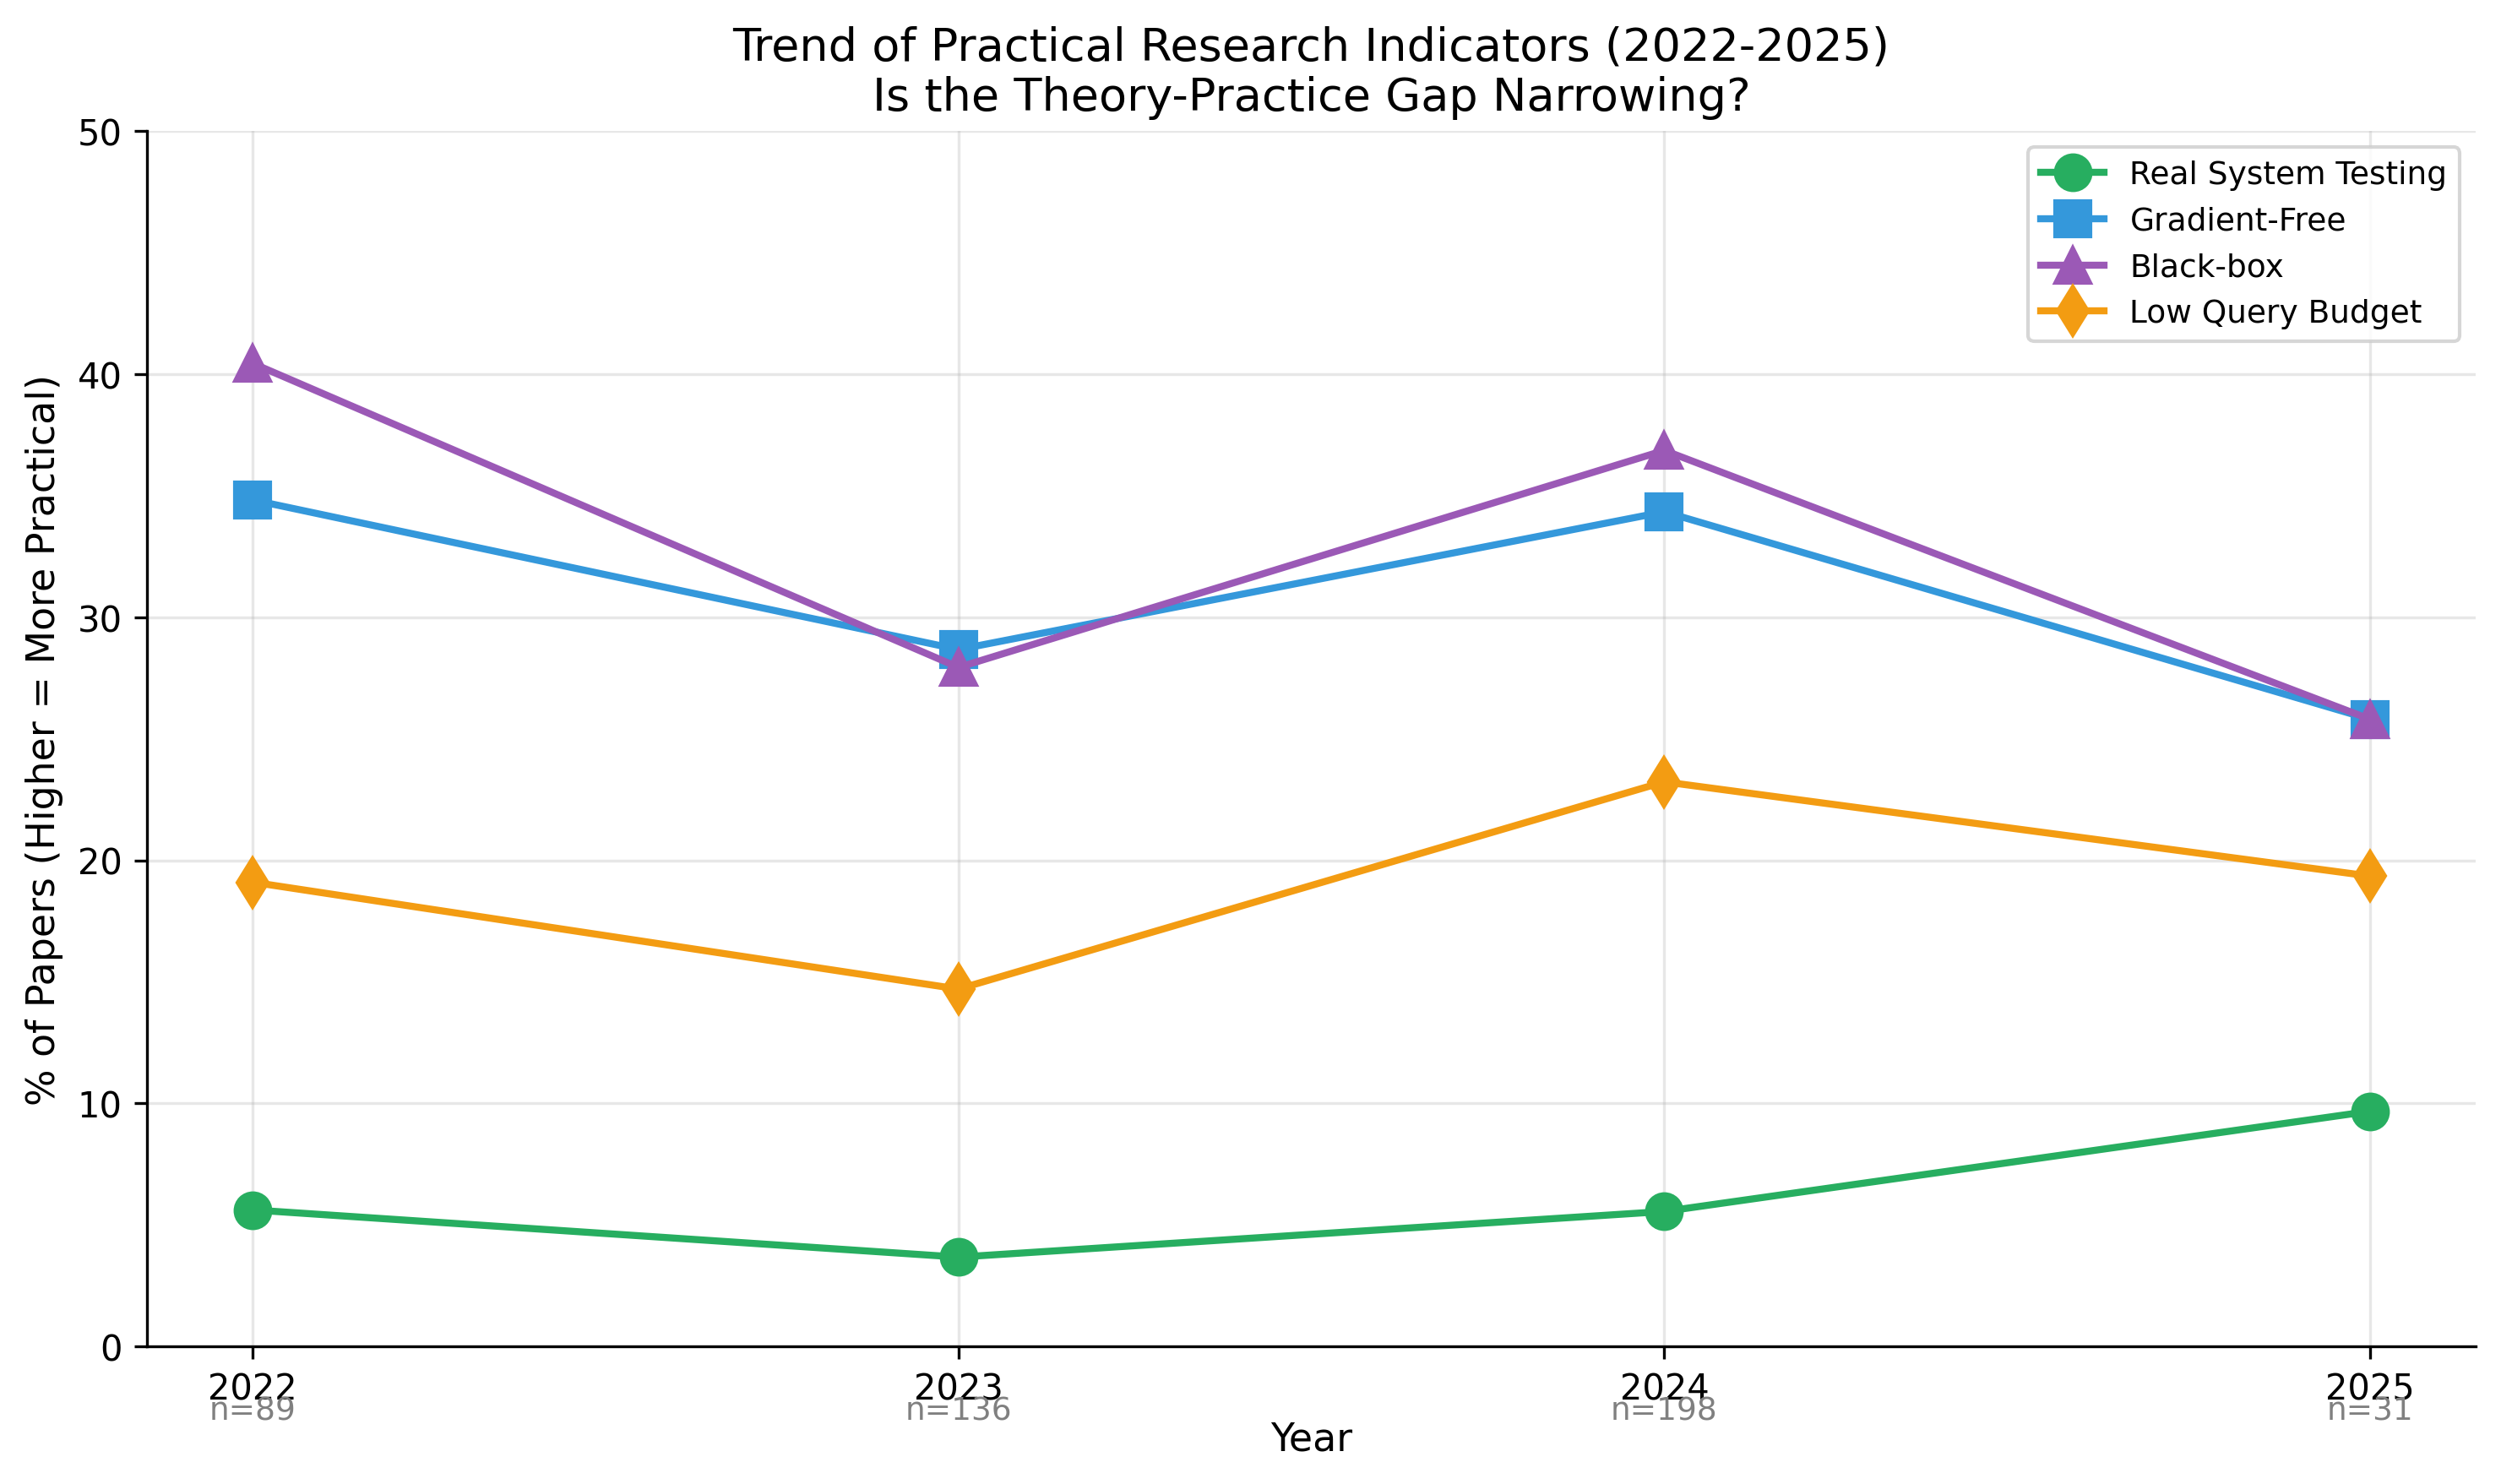
\includegraphics[width=\textwidth]{fig11_yearly_trends.png}
    \caption{Temporal trends on key gap indicators from 2022 to 2025}
    \label{fig:trends}
\end{figure}

Real-world testing remained near 5\% across all years, while gradient dependency stayed high at approximately 67 to 69\%. White-box assumptions remained dominant at 60 to 64\%, and high query budgets declined only slightly from approximately 80\% to the mid-70s by 2025. Domain bias persisted with image data dominating approximately 65\%, and economic analysis remained below 12\% without meaningful increase. Logistic regression with year as predictor confirms no statistically significant temporal trends for any indicator (all p $>$ 0.28), supporting the conclusion that the gap has not meaningfully narrowed since the Apruzzese et al.\ critique.

\clearpage
%==============================================================================
\section{Cross-Venue Analysis}
\label{sec:venues}

While all four venues exhibited similar overall patterns (chi-square tests: all p $>$ 0.20), each demonstrated distinct emphases (Fig.~\ref{fig:heatmap}). CCS papers frequently addressed model theft, watermarking, and human factors within broader system contexts. S\&P publications featured systematic evaluations with explicit threat model justification. NDSS papers often explored physical-world attacks and federated learning, grounding evaluations in realistic settings. USENIX contributed the largest volume across diverse topics, with several papers testing on real platforms.

Comparing attack- and defense-oriented papers (Fig.~\ref{fig:atk_def}), attack papers showed significantly higher gradient dependency (72.7\% vs. 59.4\%, p = 0.004) and query budgets (90.0\% vs. 64.6\%, p $<$ 0.001). However, both categories showed similarly low rates of real-system testing (approximately 5\%, p = 0.832), indicating the gap persists regardless of research focus.

\begin{figure}[!htbp]
    \centering
    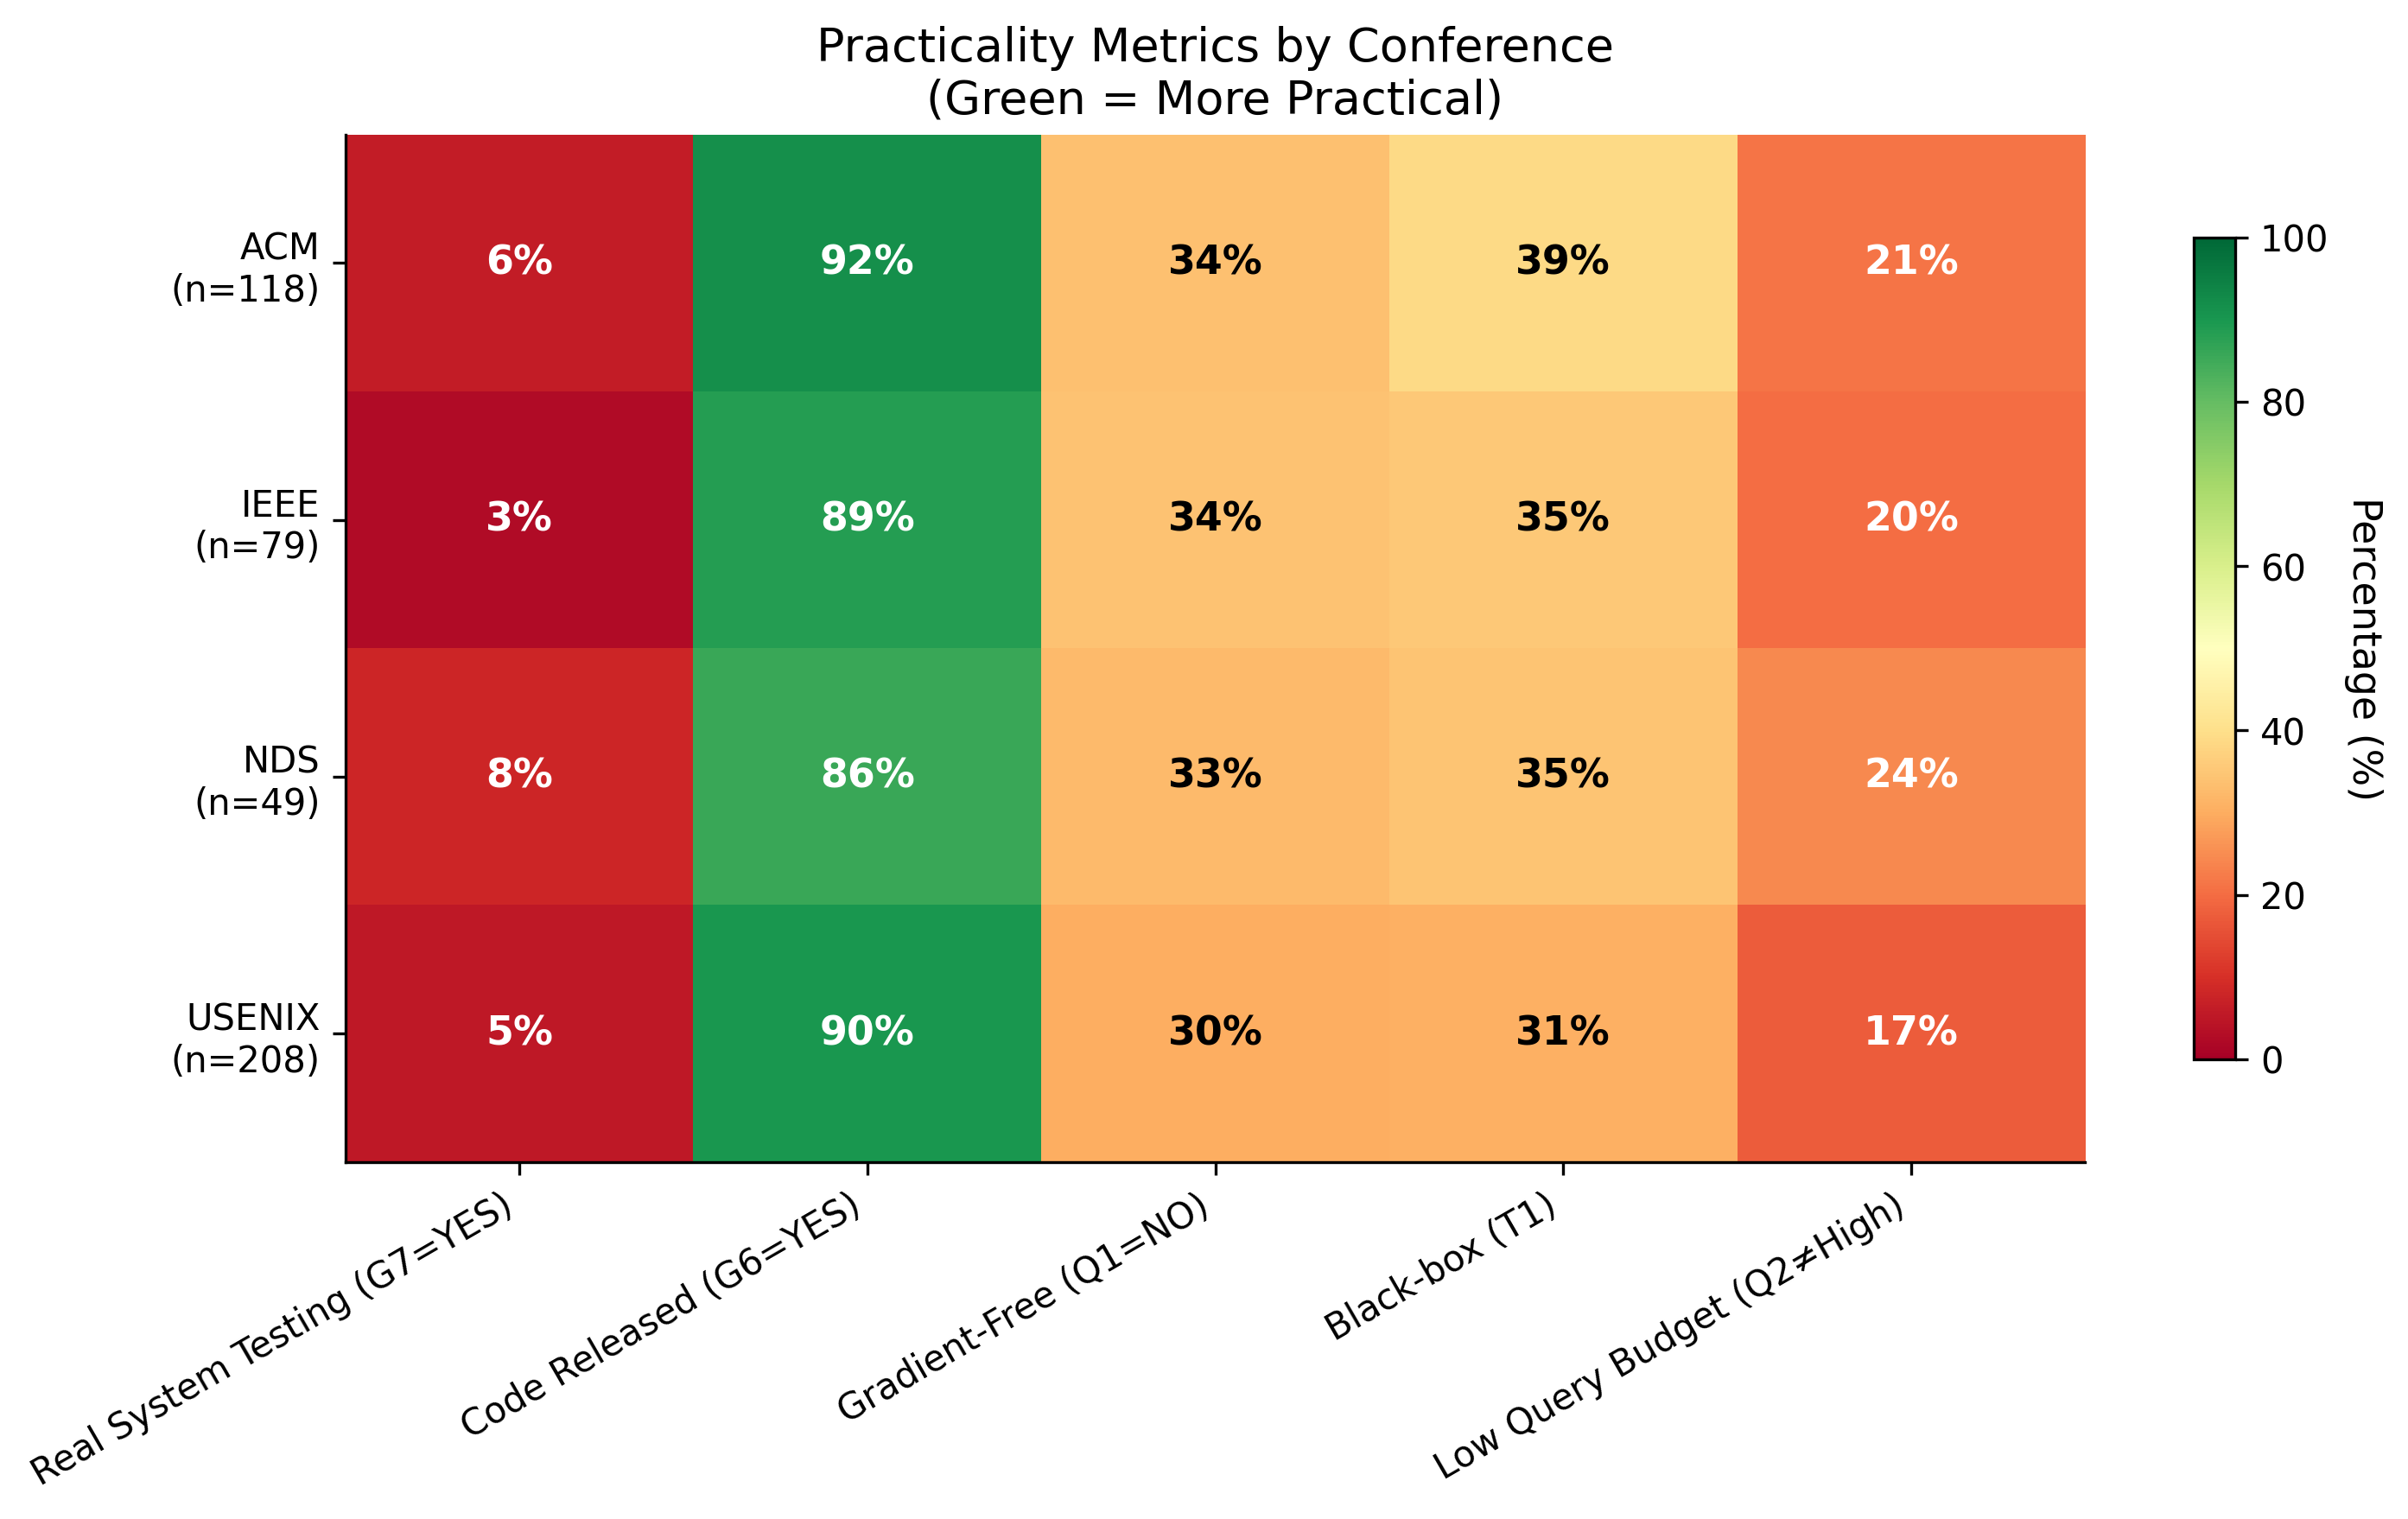
\includegraphics[width=\textwidth]{fig10_conference_comparison.png}
    \caption{Comparison of adversarial ML research characteristics across conferences}
    \label{fig:heatmap}
\end{figure}

\begin{figure}[!htbp]
    \centering
    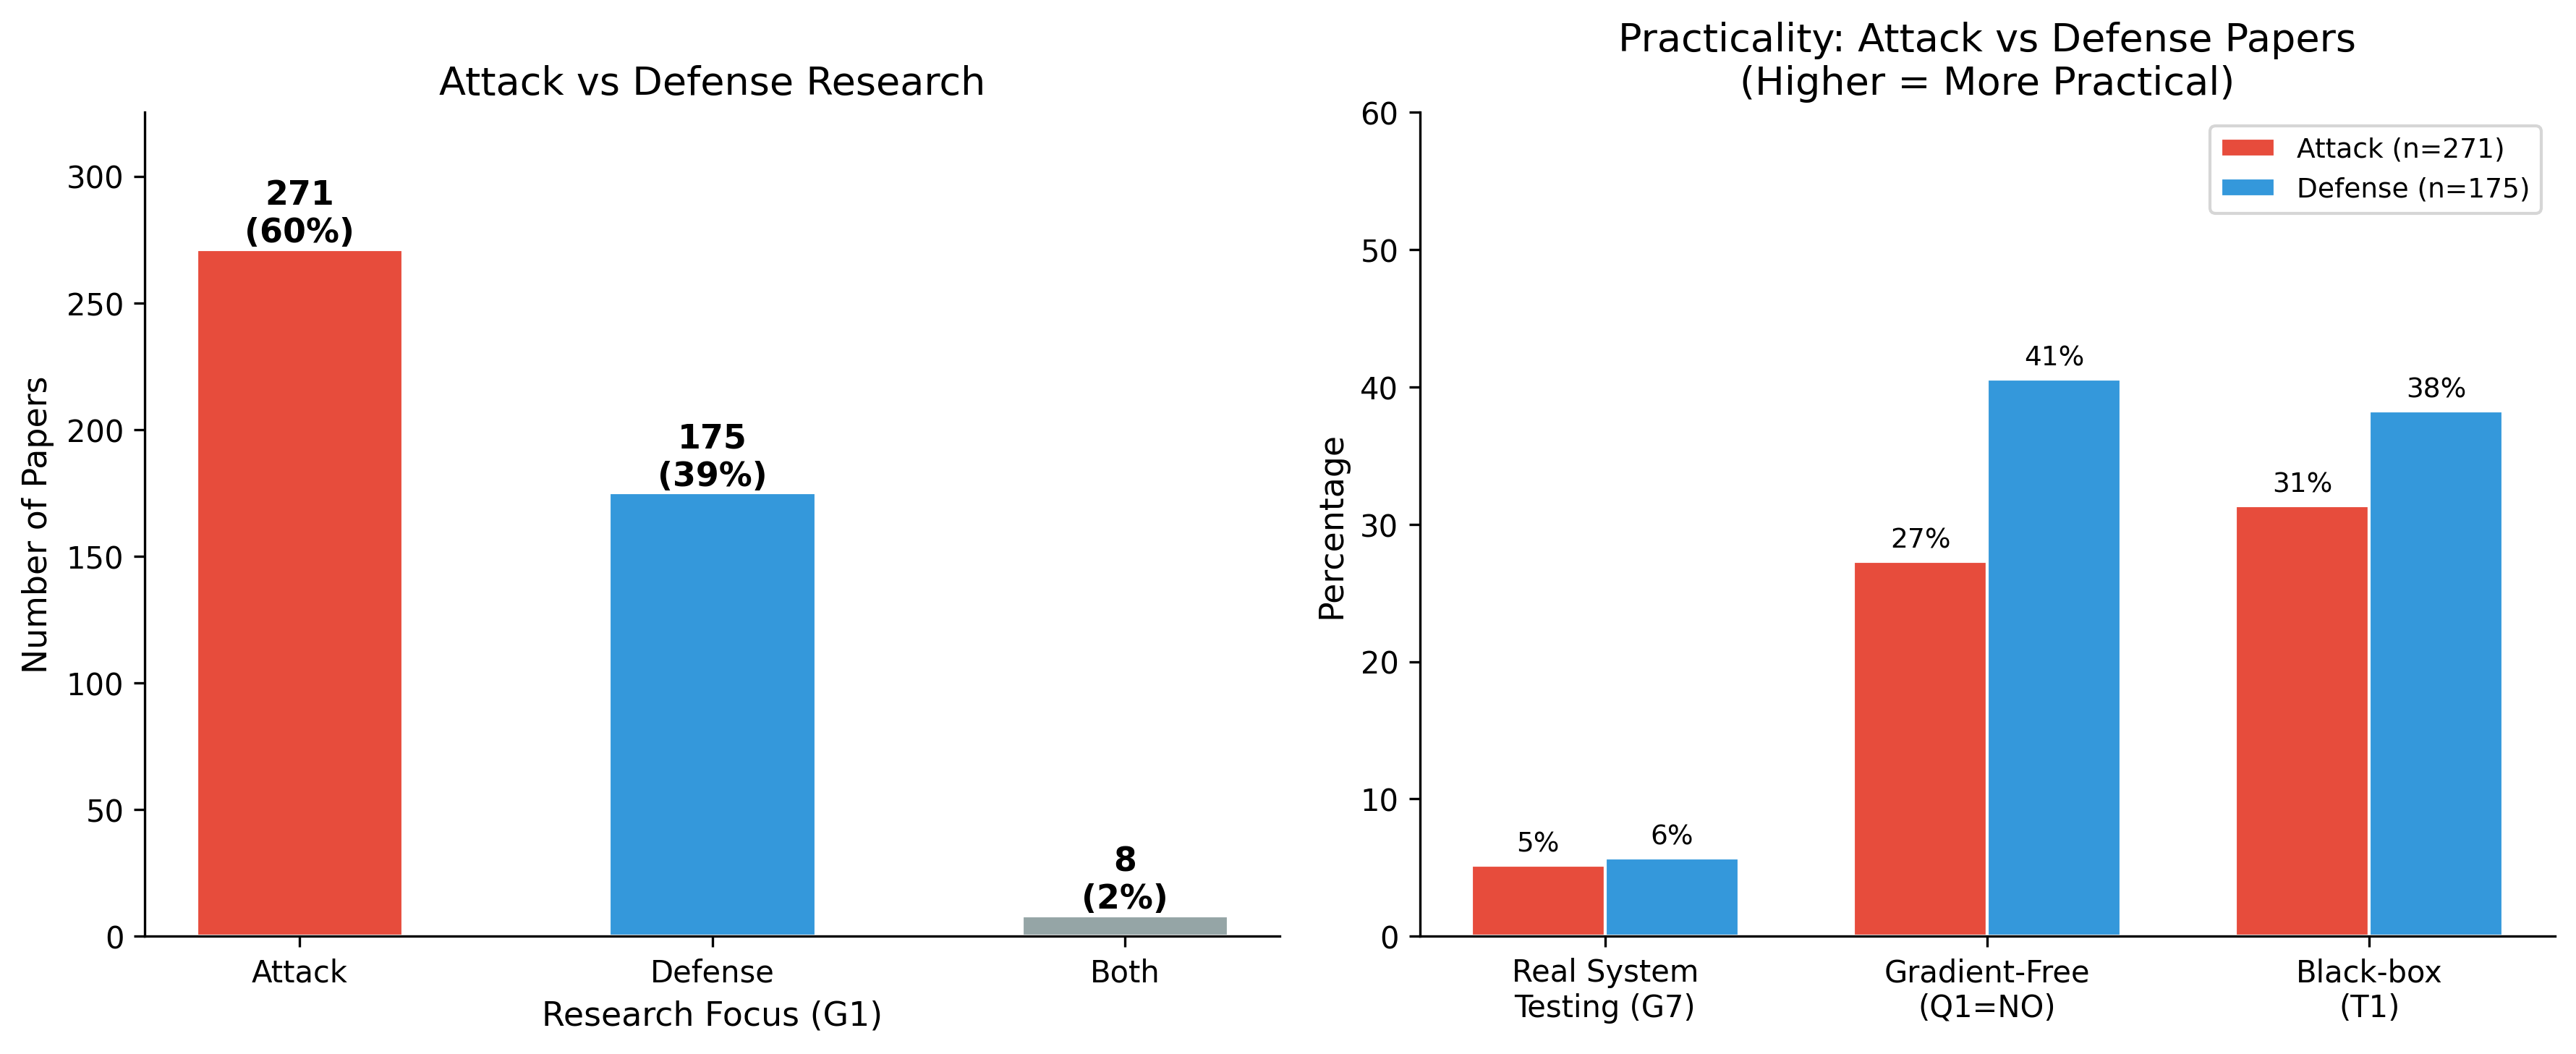
\includegraphics[width=\textwidth]{fig09_attack_vs_defense.png}
    \caption{Comparison of practicality metrics between attack- and defense-focused papers}
    \label{fig:atk_def}
\end{figure}

%==============================================================================
\section{Recommendations}
\label{sec:recommendations}

Researchers should validate methods under deployment-like conditions including limited queries, partial knowledge, and realistic computational constraints, with explicit justification when white-box access or large query budgets are assumed. Defenses should be evaluated against adaptive adversaries with utility costs reported alongside robustness metrics, and the field would benefit from diversification beyond image classification to tabular data, graphs, time-series, and multimodal systems. Conference organizers and reviewers can more explicitly assess threat model realism in review criteria, incentivize practical work through artifact evaluation and recognition for deployed evaluations, and encourage negative results showing attacks fail under realistic constraints. Industry practitioners should adjust risk assessments for deployment realities rather than accepting laboratory success rates, prioritize defenses against realistic threats (black-box attacks, low query budgets, economically motivated adversaries), and contribute anonymized logs of real attack attempts to ground academic research in operational reality. Funders can catalyze change by requiring real-world validation in industry-academic partnerships, supporting long-term deployment studies, incentivizing replication studies validating academic claims against production systems, and creating competitions with realistic constraints that align research incentives with practical security needs.

%==============================================================================
\section{Limitations}
\label{sec:limitations}

This study has several limitations. Our focus on four security conferences may not capture patterns at ML venues (NeurIPS, ICML, ICLR) where different norms may apply. The Gap Score reduces complex trade-offs to binary decisions with equal weighting, potentially oversimplifying nuanced situations; alternative weighting schemes informed by practitioner priorities or domain-specific constraints could yield different rankings. Our threshold choices (e.g., $>$1000 queries, $>$100 GPU-hours) represent reasonable but ultimately arbitrary cutoffs, and sensitivity analysis with alternative thresholds would strengthen the findings. The coding of 454 papers was conducted using AI-assisted analysis (GPT-4o, temperature=0) to operationalize the Apruzzese et al.\ framework at scale. While this enabled systematic coverage infeasible through manual review alone, it introduces potential classification errors and lacks formal inter-annotator reliability measures. The reported percentages should be interpreted as estimates rather than precise measurements. The field evolves rapidly; our dataset ends in early 2025, and research distributions may shift as technology and attacker capabilities evolve. The real-world incidents cited serve as illustrative examples rather than systematic evidence. Despite these caveats, this synthesis of quantitative trends and qualitative themes provides useful orientation for understanding the state of adversarial ML research and its relationship to deployment realities.

%==============================================================================
\section{Conclusion}
\label{sec:conclusion}

Our systematic analysis of 454 adversarial ML papers published from 2022 through 2025 reveals that the theory-practice gap identified by Apruzzese et al.\ has not meaningfully narrowed. The quantitative evidence is stark: 94.7\% of papers never test on real systems, 67.8\% require gradients that real attackers lack, 80.4\% assume query budgets that deployed systems do not allow, and 63.2\% assume white-box access that real deployments do not provide. The average Gap Score of 3.17 out of 6 indicates the typical paper makes roughly half of the impractical assumptions we measured.

Real-world adversarial incidents, from AI-orchestrated cyber espionage to prompt injection in enterprise tools, demonstrate that operational threats exploit system integration, automation, and human trust rather than gradient-based optimization. Bridging the theory-practice gap requires coordinated structural changes: realistic threat models as defaults, incentivized real-world validation, domain diversification, and consideration of economic and human factors.

The complete coded dataset of all 454 papers, along with the full codebook, GPT-4o prompts, Python analysis scripts, and figure generation code, will be provided as supplementary material and made publicly available on GitHub upon acceptance under an open license. The dataset includes paper metadata, raw coding labels for all 12 dimensions, computed Gap Scores, and statistical analysis results.

%==============================================================================
\begin{credits}
\subsubsection{\discintname}
The authors have no competing interests to declare that are relevant to the content of this article.
\end{credits}

\bibliographystyle{splncs04}
\bibliography{ref}

%==============================================================================
\appendix

\section*{Appendix}

\section{Coding Framework (Codebook)}
\label{appendix:codebook}

Table~\ref{tab:codebook} presents the complete coding framework with 12 dimensions organized into three categories: General (G1--G7), Threat Model (T1--T2), and Query/Computation (Q1--Q3). Each dimension specifies allowed values and operational definitions used for systematic classification.

\begin{table}[htbp]
\caption{Complete coding framework with 12 dimensions, allowed values, and operational definitions}
\label{tab:codebook}
\centering
\small
\begin{tabular}{llp{4cm}p{5cm}}
\hline
\textbf{ID} & \textbf{Dimension} & \textbf{Options} & \textbf{Definition} \\
\hline
G1 & Focus & atk, def, both & Attack paper, defense paper, or both \\
G2 & Attack Type & Evasion, Poisoning, Privacy, Multiple, NA & Test-time, training-time, membership/extraction, multiple types, or defense-only \\
G3 & ML Type & DL, Traditional, Both & Deep learning, classical ML, or both \\
G4 & Data Type & Images, Text, Audio, Malware, Other & Primary data modality evaluated \\
G5 & Economics & YES, NO & Any mention of cost, resources, or economics \\
G6 & Code Released & YES, NO & Source code publicly available \\
G7 & Real System & YES, NO & Tested on deployed/commercial/production system (not academic datasets) \\
T1 & Model Knowledge & White-box, Gray-box, Black-box & Full model access, partial/surrogate, or no model knowledge \\
T2 & Training Data & Full, Partial, None & Complete access, subset/surrogate, or no training data \\
Q1 & Gradients & YES, NO & Method requires gradient computation \\
Q2 & Query Budget & High, Low, None & $>$1000 queries, $<$1000 queries, or no queries \\
Q3 & Computation & High, Low & GPU/significant time vs. CPU/quick execution \\
\hline
\end{tabular}
\end{table}

The Gap Score is computed by summing six binary flags: (1) white-box assumption (T1=White-box), (2) gradient requirement (Q1=YES), (3) high query budget (Q2=High), (4) high computation (Q3=High), (5) no real-system testing (G7=NO), and (6) no economic consideration (G5=NO). Scores range from 0 (fully aligned with practical constraints) to 6 (entirely idealized assumptions).

\section{GPT-4o Analysis Prompt}
\label{appendix:prompt}

Each paper was analyzed using the following structured prompt with GPT-4o (temperature=0):

\begin{small}
\begin{verbatim}
You are analyzing an adversarial machine learning research paper.
Answer ONLY with the exact options provided.

PAPER:
Title: [paper title]
Abstract: [paper abstract]
Full Text: [complete paper text extracted via PyPDF2]

ANSWER THESE 12 QUESTIONS WITH ONLY THE SPECIFIED OPTIONS:

G1. Focus - Main contribution?
OPTIONS: atk, def, both
ANSWER: [atk for attack paper, def for defense paper, both for combined]

G2. Attack Type - What kind of attack/threat?
OPTIONS: Evasion, Poisoning, Privacy, Multiple, NA
ANSWER: [Evasion=test-time, Poisoning=training-time, 
         Privacy=membership/extraction, Multiple=several types, 
         NA=defense only]

G3. ML Type - Machine learning approach?
OPTIONS: DL, Traditional, Both
ANSWER: [DL=deep learning only, Traditional=classical ML, Both=both types]

G4. Data Type - What data is evaluated?
OPTIONS: Images, Text, Audio, Malware, Other
ANSWER: [Pick one primary type]

G5. Economics - Cost/resources/economics mentioned?
OPTIONS: YES, NO
ANSWER: [YES if ANY mention of cost/resources/economics, NO otherwise]

G6. Code Released - Source code publicly available?
OPTIONS: YES, NO
ANSWER: [YES if code is available, NO if not mentioned or not available]

G7. Real System - Tested on real/commercial systems?
OPTIONS: YES, NO
ANSWER: [YES if tested on deployed/commercial/production system, 
         NO if only academic datasets/models]

T1. Model Knowledge - What does attacker know?
OPTIONS: White-box, Gray-box, Black-box
ANSWER: [White-box=full access to model, Gray-box=partial 
         knowledge/surrogate, Black-box=no model knowledge]

T2. Training Data - Attacker's training data access?
OPTIONS: Full, Partial, None
ANSWER: [Full=complete access, Partial=subset/surrogate data, 
         None=no training data]

Q1. Gradients - Requires computing gradients?
OPTIONS: YES, NO
ANSWER: [YES if method requires gradient computation, 
         NO if gradient-free]

Q2. Query Budget - How many queries needed?
OPTIONS: High, Low, None
ANSWER: [High=>1000 queries, Low=<1000 queries, None=no queries needed]

Q3. Computation - Computational resources needed?
OPTIONS: High, Low
ANSWER: [High=needs GPU/significant time, Low=CPU ok/quick execution]

CRITICAL INSTRUCTIONS:
- Answer ONLY with the exact option words provided
- Do not add explanations
- Format EXACTLY as shown below
- If unclear from text, make best judgment

REQUIRED FORMAT:
G1: [answer]
G2: [answer]
...
Q3: [answer]
\end{verbatim}
\end{small}

\end{document}
